
\documentclass[journal,comsoc]{IEEEtran}
\usepackage[T1]{fontenc}% optional T1 font encoding
\usepackage[english]{babel}



% *** CITATION PACKAGES ***
\usepackage{cite}
\usepackage{color}
% *** GRAPHICS RELATED PACKAGES ***
%
\ifCLASSINFOpdf
   \usepackage[pdftex]{graphicx}

\else
  
  \usepackage[dvips]{graphicx}
  
\fi

% *** MATH PACKAGES ***
%
\usepackage{amsmath}
\interdisplaylinepenalty=2500
\usepackage[cmintegrals]{newtxmath}
\usepackage{bm}
\usepackage{graphicx}


% *** SPECIALIZED LIST PACKAGES ***
\usepackage{algorithmic}

% *** ALIGNMENT PACKAGES ***
\usepackage{array}

% *** LOREM LIPSUM PACKAGE ***
\usepackage{lipsum}  

% *** SUBFIGURE PACKAGES ***
\ifCLASSOPTIONcompsoc
  \usepackage[caption=false,font=normalsize,labelfont=sf,textfont=sf]{subfig}
\else
  \usepackage[caption=false,font=footnotesize]{subfig}
\fi

% *** FLOAT PACKAGES ***
\usepackage{fixltx2e}
\usepackage{dblfloatfix}

\ifCLASSOPTIONcaptionsoff
  \usepackage[nomarkers]{endfloat}
 \let\MYoriglatexcaption\caption
 \renewcommand{\caption}[2][\relax]{\MYoriglatexcaption[#2]{#2}}
\fi

% *** PDF, URL AND HYPERLINK PACKAGES ***
\usepackage{url}

% correct bad hyphenation here
\hyphenation{op-tical net-works semi-conduc-tor}


%%%%%%%%%%%%%%%%%
%%% Commandes %%%
%%%%%%%%%%%%%%%%%

%%% Physique %%%
\newcommand{\cst}{\text{cst}}
\newcommand{\E}{\vec E}
\newcommand{\B}{\vec B}
\newcommand{\F}{\vec F}
\newcommand{\module}[1]{\left|#1\right|}
\newcommand{\EX}[1]{\mathbb{E} \left[#1\right]}% expected value
\newcommand{\HE}{\textbf{H}_{\text{E}}}
\newcommand{\HB}{\textbf{H}_{\text{B}}}
\newcommand{\vb}{\textbf{v}_{\text{B}}}
\newcommand{\ve}{\textbf{v}_{\text{E}}}
\newcommand{\spread}{\textbf{S}}
\newcommand{\SH}{\textbf{S}^H}
\newcommand{\w}{\textbf{w}}

%%% Math %%%

\newcommand{\vect}[1]{\boldsymbol{\mathrm{#1}}}
\newcommand{\mat}[1]{\boldsymbol{\mathrm{#1}}}
\newcommand{\rot}{\text{rot}\,}
\newcommand{\divv}{\text{div}\,}
\newcommand{\phas}[1]{\underline{#1}}
\newcommand{\RE}{\text{Re}}
\newcommand{\R}{\mathbb{R}}
\newcommand{\C}{\mathbb{C}}
\usepackage{xfrac}
\newcommand\independent{\protect\mathpalette{\protect\independenT}{\perp}}
\def\independenT#1#2{\mathrel{\rlap{$#1#2$}\mkern2mu{#1#2}}}

\renewcommand{\d}[1]{\ensuremath{\operatorname{d}\!{#1}}}

\usepackage{hyperref}


\usepackage{tabularx}
\newcolumntype{L}{>{\raggedright\arraybackslash}X}
%%%%%%%%%%%%%%%%% BEGINNING OF THE TEXT %%%%%%%%%%%%%%%%%%%%%%%%%





\begin{document}
	
\title{Physical Layer Security in Frequency-Domain Fast-Fading TDD Time-Reversal SISO OFDM Communication}

\author{\IEEEauthorblockN{Sidney J. Golstein\IEEEauthorrefmark{1}\IEEEauthorrefmark{2},
		Trung-Hien Nguyen\IEEEauthorrefmark{1},
		Fran\c cois Rottenberg\IEEEauthorrefmark{1},
		Fran\c cois Horlin\IEEEauthorrefmark{1}, 
		Philippe De Doncker\IEEEauthorrefmark{1}, and
		Julien Sarrazin\IEEEauthorrefmark{2}} \\
\IEEEauthorblockA{\IEEEauthorrefmark{1}Wireless Communication Group,
	Universit\'{e}  Libre de Bruxelles, 1050 Brussels, Belgium} \\
\IEEEauthorblockA{\IEEEauthorrefmark{2}Sorbonne Université, CNRS, Laboratoire de Génie Electrique et Electronique de Paris, 75252, Paris, France \\
	Université Paris-Saclay, CentraleSupélec, CNRS, Laboratoire de Génie Electrique et Electronique de Paris, 91192, Gif-sur-Yvette, France} \\
\IEEEauthorblockA{\small{\{sigolste,trung-hien,francois.rottenberg,fhorlin,philippe.dedoncker\}@ulb.ac.be}} \\
\IEEEauthorblockA{\small{julien.sarrazin@sorbonne-universite.fr}}
\thanks{This work was supported by the ANR GEOHYPE project, grant ANR-16-CE25-0003 of the French Agence Nationale de la Recherche and was also carried out in the framework of COST Action CA15104 IRACON.}}

% The paper headers
\markboth{Journal of ...,~Vol.~to-define, No.~to-define, \today}%
{Shell \MakeLowercase{\textit{et al.}}: Bare Demo of IEEEtran.cls for IEEE Communications Society Journals}


% make the title area
\maketitle


\begin{abstract}
A frequency domain (FD) fast-fading (FF) time division duplex (TDD) time-reversal (TR) precoder is proposed to perform physical layer security (PLS) in single-input single-output (SISO) system using orthogonal frequency-division multiplexing (OFDM). To maximize the secrecy of the communication, the design of an artificial noise (AN) signal well-suited to the proposed FD TR-based OFDM SISO system is derived. This new scheme guarantees the secrecy of a communication towards a legitimate user when the instantaneous channel state information (CSI) of a potential eavesdropper is not known. The instantaneous CSI of the legitimate receiver is known at the transmitter thanks to channel reciprocity  in TDD systems. In particular, we derive an AN signal that does not corrupt the data transmission to the legitimate receiver but degrades the decoding performance of the eavesdropper. We consider three possible decoding structures at the eavesdropper position depending on the handhsake procedure, and we derive closed-form approximations of the AN energy to inject in order to maximize the secrecy rate (SR) of the communication. Furthermore, a waterfilling-like power allocation strategy, keeping into account the AN injection, is presented to further enhance the secrecy of the scheme. Simulation results are presented to demonstrate the security performance of the proposed secure FD TR SISO OFDM system.
\end{abstract}

% Note that keywords are not normally used for peerreview papers.
\begin{IEEEkeywords}
Physical layer security, time-reversal, time division duplex, fast-fading, eavesdropper, SISO-OFDM, artificial noise, waterfilling, secrecy rate.
\end{IEEEkeywords}

\IEEEpeerreviewmaketitle





%%%%%%%%%   INTRODUCTION   %%%%%%%%% 
\section{Introduction}
%\IEEEPARstart{T}{his} demo file is intended to serve as a ``starter file''
%for IEEE Communications Society journal papers produced under \LaTeX\ using
%IEEEtran.cls version 1.8b and later.
% You must have at least 2 lines in the paragraph with the drop letter
% (should never be an issue)
%I wish you the best of success.


\IEEEPARstart{T}{he} demand for wireless communication services and the number of interconnected users is increasing day by day. Internet-based services have become indispensable in daily life. Wireless media has become the dominant access for most of these services and is intrisically unsecure due to its broadcast nature. Therefore, several issues have emerged and need to be urgently adressed such as data confidentiality and integrity, \cite{8509094,8543573}.

% Parler de crypto et ses prob
The concept of security started in Shannon's work, \cite{6769090}. First, these techniques are based on the assumption that the eavesdropper (Eve) has limited computational power capabilities. With the fast development in computing power devices, secret keys that were secure decades ago are nowadays more subject to successful brut-force attacks. Second, the security is enhanced when the key length increases, resulting in more waste of resources. In addition, the key management processes become a real issue with the deployment of large-scale heterogeneous and decentralized networks involving different acces technologies, such as 5G networks. Finally, the emergence of power-limited, delay-sentive and processing-restricted wireless technologies, such as Internet Of Things (IoT), banking, health monitoring, vehicular communications, makes cryptography-based methods naturally unsuitable, \cite{8509094}.

% Prob de la crypto assurés par la PLS
To circumvent the aforementionned issues, physical layer security (PLS) has emerged as an effective way to enhance security of wireless communications, \cite{alves2012performance,yang2012physical,tran2015secrecy,8353879}. PLS classically takes benefit of the characteristics of wireless channels (e.g., multipath fading, noise, dispersion, diversity) to improve security of communications against potential eavesdroppers without relying on computational complexity, i.e., the security will not be affected if Eve has unlimited computing capabilities, \cite{9049811,snchez2020survey}. 

% Introduction de la PLS
The starting point of PLS was exposed in 1975 by Wyner where it is explained that a communication can be made secure, without sharing a secret key, when the wiretap channel of the eavesdropper is a degraded version, i.e., noisier, of the legitimate link (Bob), \cite{6772207}. This work was later extended to the broadcast channel in \cite{1055892} and to the Gaussian channel in \cite{1055917}. 

% SINR based PLS avec ses hypothèses et ses métriques principales: une des grande classes de la PLS
It is of prime importance to evaluate the effectiveness of a PLS scheme by quantifying the degree of secrecy it can provide with a suitable metric. One of the most studied class of PLS metrics is the secrecy capacity. The information-theoretic secrecy-capacity is defined as the number of bits per channel use that can be reliably transmitted from a legitimate transmitter (Alice) to a legitimate receiver (Bob) while guaranteeing a negligible information leakage to the eavesdropper (Eve), \cite{bloch_barros_2011}.

PLS performance highly depends on the availability of channel state information (CSI) at the communication parties. It is generaly assumed that the transmitter (Alice) knows Bob CSI but does not know or partially knows Eve CSI , since she is considered as passive, \cite{8509094}. We often assume Eve as an external passive node of the network that tries to eavesdrop the data. We usually consider that Bob and Eve CSI's are spatially independent. PLS can be achieved by increasing the SINR at the intended position and decreasing the SINR at the unintended position. This can be done by designing a suitable channel-based adaptive transmission scheme and/or by injecting an artificial noise (AN) signal to the data. These techniques can be implemented in the space, time and/or frequency domains, \cite{8509094,7762075,MELKI20191}.

% Parler des SINR based-PLS : channel coding/channel adaptation/signal jamming
Channel-based adaptation secrecy schemes were first introduced in \cite{4529264,4529282,4626059}. In these works, it was proven that positive secrecy can be obtained even if, on average, the channel between Alice and Bob is a degraded version of the one between Alice and Eve, by optimizing or adapting at the transmitter side the communication parameters. In doing so, the transmitted signal will be optimal for Bob's channel and not for Eve's one since they experience different fading. The concept of AN addition was first established in \cite{1558439,1605889,4543070}. The idea is to made Eve's channel condition artificially degraded by intentionnaly adding an AN signal at the transmitter side. This AN signal does not degrade Bob's channel, therefore leading to a PLS enhancement, \cite{8509094}


While many works implement these schemes using multiple antennas at the transmitter, via frequency diverse array beamforming \cite{li_qiang_2018_1159254,8078202}, directional modulation (DM) \cite{5159486},  antenna subset modulation (ASM) \cite{6544472}, near-field direct antenna modulation (NFDAM) \cite{4684619,4523120}, multiple-inputs multiple-outputs (MIMO) diversity \cite{5580113,7070667,8786136,5738303},... few ones do it using single-input single-output (SISO) systems \cite{li2013waveform,9003692,8093595,8093591,xu2018security,li2018artificial,li2017artificial,9049811,7475864,7041552}.  In \cite{9062307}, the information-theoretic secrecy capacity of an Offset-QAM-based filterbank multicarrier (FBMC-OQAM) communication over a wiretap frequency selective channel is studied. The authors compare the secrecy capacity of the FMBC-OQAM modulation with a cyclic prefix-orthogonal frequency-division multiplexing (CP-OFDM) modulation. In \cite{li2013waveform}, a symbol waveform optimization technique in time-domain (TD) is proposed to reach a desired SINR at Bob with AN injection, under power constraint, when eavesdropper’s CSI is not known. Another approach to increase the SINR in SISO systems is time reversal (TR) pre-filtering. This has the advantage to be implemented with a simple precoder at the transmitter. TR achieves a focusing gain at the intended receiver position only, thereby naturally offering intrinsic anti-eavesdropping capabilities, \cite{9003692,oestges2005characterization}. TR is achieved by up/downsampling the signal in the TD. While the impact of the back-off rate (BOR), defined as the up/downsampling rate \cite{dubois2010use}, was studied in \cite{9003692,9049811}, very basic decoding capabilities were attributed at Eve. TR can also be equivalently implemented in frequency domain (FD) by replicating and shifting the signal spectrum, \cite{8883213}. FD implementation has the advantage to be easily performed using orthogonal frequency-division multiplexing (OFDM). In \cite{8093595,8093591} FD OFDM schemes are presented consisting of subcarriers index selection. Only several subcarriers are used for data transmission depending on their channel gains.

To further enhance the secrecy, few works combine TD or FD precoding with AN injection, \cite{xu2018security,li2018artificial,li2017artificial,7475864,7041552}. In \cite{xu2018security,li2018artificial,li2017artificial}, TD TR precoders are presented. In these works, the AN is added either on all the channel taps or on a set of selected taps. While the condition for AN generation is given, its derivation is however not detailed. In \cite{7475864,7041552}, FD precoders using OFDM and AN injection are presented. The idea is to use several OFDM subcarriers for dummy data transmission, i.e., several subcarriers are used for data obfuscation. However, the encryption information must be shared between the transmitter and the legitimate receiver, leading to more processing needed at the receiver. In addition, the security is enhanced when more subcarriers are used for data obfuscation, at the expense of the data rate. Furthermore, it is assumed that Eve has no knowledge about the legitimate link.

% Motivation de notre article
In this article, we present an original and novel FD TR precoder in SISO OFDM systems with AN addition,  which establish secure communications. The paper is an extension of the study in \cite{9049811} where only one decoding capability was considered at the wiretap link. In the following, we investigate three scenarios corresponding to three different eavesdropper knowledges depending on the handshake procedure.  Bob's CSI is fully known at Alice, using channel reciprocity inherent from time division duplex (TDD) systems, in a fast fading (FF) environment. An AN signal is designed in the FD to maximize the ergodic SR of the communication in the presence of a passive eavesdropper whose instantaneous CSI is supposed unknown. A power allocation technique, keeping into account the AN injection, is also derived in order to further enhance the communication SR. The proposed scheme uses only frequency diversity inherently present in multipath environments to achieve security. It can therefore be used in SISO systems and is then well-suited for resource-limited nodes such as encountered in IoT or vehicular communications for instance, \cite{9049811}. In addition, the presented scheme does not suppose any degradation of Eve's channel compared to the legitimate link. Furthermore, the OFDM implementation makes this approach compatible with LTE and 5G networks.

% Structure de l'article.
The reminder of this article is organized as follows: the handshake and the communication protocols are exposed in Section \ref{sec:system-model}. Section \ref{sec:perf} presents a closed-form approximation of the amount of AN energy to be injected in order to maximize the SR, for the different decoding structures at Eve. A derivation of the required SNR at Bob to target a desired SR is proposed, as a function of the communication parameters. Then, a waterfilling optimization procedure is outlined in order to further increase the communication SR. Theoretical and numerical results are shown in Section \ref{sec:simulation-results}. Section \ref{sec:conclusions} concludes the paper.

% Notation
\textit{\textbf{Notation:}} the italic lower-case letter denotes a complex number. Greek letter corresponds to a scalar, the bold lower-case letter denotes a column vector. Bold upper-case letter corresponds to a matrix; $\textbf{I}_N$ is $N \times N$ identity matrix; $(.)^{-1}$, $(.)^{*}$, $(.)^{H}$ are respectively the inverse, the complex conjugate and the Hermitian transpose operators; $\EX{.}$ is the expectation operator; $\module{.}$ is the modulus operator (element-wize modulus if we deal with a matrix); $\odot$ is the element-wize (hadamard) product between two vectors of same dimension.







%%%%%%%%%   SYSTEM MODEL   %%%%%%%%% 
\section{System Model}\label{sec:system-model}


\subsection{Communication Protocol}
In order to transmit secure data between Alice and Bob, the useful data will be precoded and an AN signal $\w$ will be added to it before transmission, as depicted in Fig.\ref{fig_com_scheme}.  
\begin{figure}[h!t]
	\centering
	\includegraphics[width=1\linewidth]{graphs/com_scheme_an.PNG}
	\caption{Communication scheme}
	\label{fig_com_scheme}
\end{figure}\\
The system model was already described in \cite{9049811}. Briefly, it consists in data transmission onto OFDM blocks with $Q$ subcarriers. We consider that only one data block $\textbf{x}$ is sent and is composed of $N$ symbols $x_n$ (for $n = 0,..., N-1$, with $N\leq Q$). The symbol $x_n$ is  a zero-mean random variable (RV) with variance $\EX{|x_n|^2} = \sigma_x^2 = 1$, i.e., a normalized constellation is considered. The block is then spread by a factor $U = Q/N$, called back-off rate (BOR), thanks to the spreading matrix $\spread$ of size $Q\times N$. The design of the spreading matrix is such that it allows not to increase the PAPR, as suggested in \cite{4394231}. The matrix is expressed in \cite{9049811}. The signal is spread in the FD by repetiting and shifting its spectrum,\cite{8883213}. In doing so, each data symbol will be transmitted onto $U$ different subcarriers with a spacing of $N$ subcarriers, introducing frequency diversity. The spread sequence is then precoded with the complex conjugate of Bob's channel $\HB^*$, before addition of the AN signal $\textbf{w}$  and transmission. 

The AN should not have any impact at Bob's position but should be seen as interference everywhere else since Alice does not have any information about Eve's instantaneous CSI, i.e., Eve is a passive node. Furthermore, this signal should not be guessed at the unintended positions to ensure the secure communication. From that, the idea of the AN signal addition is to corrupt the data detection everywhere except at Bob's position. With these considerations, the transmitted sequence becomes:
\begin{equation}
	\textbf{x}_{\text{TR}} = \sqrt{\alpha} \;\HB^*  \spread\; \textbf{x} +  \sqrt{1-\alpha} \; \w
	\label{eq:sym_rad_AN}
\end{equation} 
where $\alpha \in [0,1]$ defines the ratio of the total energy sent dedicated to the useful signal, knowing that $\EX{\module{\w}^2} = \EX{\module{\HB^*\spread\textbf{x}}^2} =  1/\vect{U}$. Whatever the value of $\alpha$, the total transmitted power remains constant.

In order to precode the data, Alice needs to have the knowledge of Bob CFR. We consider that Alice can perfectly estimate Bob CFR. The channels between Alice and Bob ($\HB$) and between Alice and Eve ($\HE$) are assumed to be static during the transmission of one OFDM symbol. However, the CFRs differ between two subsequent OFDM blocks thanks to the FF hypothesis. We assume that $\HB$ and $\HE$ are $Q\times Q$ diagonal matrices whose elements are $h_{\text{B},q}$ and $h_{\text{E},q}$ (for $q = 0,...,Q-1$) follow a zero-mean unit-variance complex normal distribution, i.e., their modulus follow a Rayleigh distribution. We also consider that the overall channel energies are normalized to unity for each channel realization, i.e., $\mathbb{E}\left[\left|h_{\text{B},q}\right|^2\right]  = \mathbb{E}\left[\left|h_{\text{E},q}\right|^2\right] = 1, \; q = 0,...,Q-1$. The precoding matrix $\HB^*$ is also a diagonal matrix with elements $h_{\text{B},q}^*$. At Bob, a despreading operation is performed by applying $\spread^H$. We consider that Bob and Eve know the spreading sequence. Bob will then apply a ZF equalization.  As it will be explained in section \ref{sec:establishment}, three decoding structures $\textbf{G}$ will be investigated at Eve. These different schemes will lead to different level of security performances. After decoding, Eve also perfoms a ZF equalization. A perfect synchronization is finally assumed at Bob and Eve positions.\\







%
\subsubsection{Artificial noise Design}\label{sec:artificial-noise-design}
In order not to have any impact at the intended position, the AN signal must satisfy the following condition:
\begin{equation}
	\textbf{A} \w \; = \; \textbf{0}
	\label{eq:an_cond}
\end{equation}
where $\textbf{A} = \spread^H\HB\; \in \C^{N\times Q}$. Condition (\ref{eq:an_cond}) ensures that $\w$ lies in the right null space of $\textbf{A}$. If we perform a singular value decomposition (SVD) of $\textbf{A}$, we obtain:
\begin{equation}
	\textbf{A} = \textbf{U} 
	\begin{pmatrix}
		\Sigma \; \textbf{0}_{Q-N\times Q}
	\end{pmatrix}
	\begin{pmatrix}
		\textbf{V}_1^H \\
		\textbf{V}_2^H
	\end{pmatrix}
	\label{eq:an_svd}
\end{equation}
where $\textbf{U} \in \C^{N \times N}$ contains left singular vectors, $\Sigma \in \C^{N \times N}$ is a diagonal matrix containing singular values, $\textbf{V}_1 \in \C^{Q \times N}$ contains right singular vectors associated to non-zero singular values, and $\textbf{V}_2 \in \C^{Q \times Q-N}$ contains right singular vectors that span the right null space of $\textbf{A}$. Therefore, the AN signal can be expressed as:
\begin{equation}
	\w = \beta \textbf{V}_2 \tilde{\w}
	\label{eq:an_w}
\end{equation}
which ensures that (\ref{eq:an_cond}) is satisfied for any arbitrary vector $\tilde{\w} \in \C^{Q-N \times 1}$. Since $Q = NU$, as soon as $U\geq 2$, there is a set of infinite possibilities to generate $\tilde{\w}$ and therefore the AN signal. In the following, we assume that $\tilde{\w}$ is a zero-mean circularly symmetric white complex Gaussian noise with covariance matrix $\EX{\tilde{\w}(\tilde{\w})^H} = \textbf{I}_{Q-N }$. The AN signal is then generated thanks to (\ref{eq:an_w}) with a weighting coefficient $\beta$ to have an energy of 1/U.


\subsubsection{Received sequence at the intended position}
After despreading, the received sequence at Bob is: 
\begin{equation}
	\textbf{y}_{\text{B}}^H = \sqrt{\alpha} \; \spread^H \module{\HB}^2 \spread \textbf{x} \;  +  \;  \spread^H \textbf{v}_\text{B} 
	\label{eq:rx_bob_AN}
\end{equation}

where $\textbf{v}_\text{B}$ is the FD complex AWGN. The noise's variance is $\EX{|v_{\text{B},n}|^2}  = \sigma_{\text{V,B}}^2$ and the covariance matrix is $\EX{(\spread^H  \textbf{v}_\text{B}) . (\spread^H \textbf{v}_\text{B})^H} = \sigma_{\text{V,B}}^2 . \textbf{I}_N$. We also assume that the data and noise symbols,  $x_n$ and $v_{\text{B,n}}$ respectively, are independent of each other. In (\ref{eq:rx_bob_AN}), each transmitted symbol is affected by a real gain at the position of the legitimate receiver. This results from the data precoding at Alice leading to the product $\HB\HB^*$ in the received sequence at Bob, which is a real diagonal matrix. The gains differ between each symbol in the OFDM block but increases with an increase of the BOR value as each symbol would be sent on more subcarriers and would benefit from a larger frequency diversity gain. If we consider a fixed bandwidth, the TR focusing effect is enhanced for higher BOR's at the expense of the data rate. We also observe that no AN contribution is present in (\ref{eq:rx_bob_AN}) since (\ref{eq:an_cond}) is respected. A ZF equalization is performed at the receiver leading to:
\begin{equation}
	\begin{split}
		\hat{\textbf{x}}_{\text{B}} &= \left( \sqrt{\alpha} \spread^H \module{\HB}^2 \spread \right)^{-1}  \left(\sqrt{\alpha}  \spread^H\module{\HB}^2 \spread \textbf{x}   +    \spread^H \textbf{v}_\text{B}\right) \\
		&= \textbf{x} + \left( \sqrt{\alpha} \spread^H \module{\HB}^2 \spread \right)^{-1} \spread^H \textbf{v}_\text{B}
	\end{split}
	\
	\label{eq:rx_bob_AN_eq}
\end{equation}
From (\ref{eq:rx_bob_AN_eq}), a perfect data recovery is possible in high SNR scenarios.



%
\subsubsection{Received sequence at the unintended position}
The received sequence at the eavesdropper position is given by:
\begin{equation}
	\textbf{y}_{\text{E}}^G = \sqrt{\alpha}  \textbf{G} \HE \HB^* \spread\textbf{x} + \sqrt{1-\alpha} \textbf{G} \HE \w + \textbf{G}  \textbf{v}_\text{E}
	\label{eq:rx_eve_an}
\end{equation}
where $\textbf{G}$ is a $N \times Q$ decoding matrix performed by Eve, $\textbf{v}_\text{E}$ is the complex AWGN. The nature of the decoding matrix will be determined by the handshking protocols, which are presented in \ref{sec:establishment}. The noise variance is $\EX{|v_{\text{E,n}}|^2} = \sigma_{\text{V,E}}^2$.  In (\ref{eq:rx_eve_an}), $\HE \HB^*$ is a complex diagonal matrix. Therefore, since the transmitted data is precoded to reach Bob, each received symbol component will be affected by a random coefficient. This coefficient can be real or complex depending on the decoding structure $\textbf{G}$. If it is complex, its magnitude does not depend on the BOR value. It results in an absence of TR gain at the unintended position. As a consequence, worse decoding performance will be expected at Eve than at the intended position. In addition, we observe in (\ref{eq:rx_eve_an}) a term depending on the AN signal. It results from the precoding at Alice since $\textbf{G}\HE \w \neq \textbf{0}$ in general. This term introduces an interference at Eve and thus degrades the received constellation even in a noiseless environment. After ZF equalization, the estimated symbols are:
\begin{equation}
	\begin{split}
		\hat{\textbf{x}}_{\text{E}} =& \left(\textbf{G} \HE \HB^* \spread \right)^{-1}
		\left( \sqrt{\alpha} \textbf{G} \HE \HB^* \spread \textbf{x} +   \sqrt{1-\alpha} \textbf{G} \HE \w  +  \textbf{G}  \textbf{v}_\text{E}  \right) \\
		=& \;\sqrt{\alpha}\textbf{x} + \sqrt{1-\alpha} \left(\textbf{G} \HE \HB^* \spread \right)^{-1}  \textbf{G} \HE \w + \left(\textbf{G} \HE \HB^* \spread \right)^{-1}  \textbf{G} \textbf{v}_\text{E}
	\end{split}
	\label{eq:rx_an_eve_eq}
\end{equation}
Equation (\ref{eq:rx_an_eve_eq}) shows that the addition of AN in the FD TR SISO OFDM communication can secure the data transmission. Indeed, a term depending on the AN signal still remains after equalization even in high SNR scenarios. It is to be noted that, since $\w$ is generated from an infinite set of possibilities, even if Eve knows its equivalent channel $\HE\HB^*$ and the spreading sequence, she cannot estimate the AN signal  to try retrieving the data.  The degree of security will depend on the investigated scenario, i.e., decoding structure $\textbf{G}$ at Eve, and the amount of data energy (via $\alpha$) that is injected into the communication, as it will be explained in Section \ref{sec:perf}.



\subsection{Handshake Protocol}
\label{sec:establishment}
Prior to the secure data transmission between Alice and Bob, a handshake protocol must take place. Depending on it, Eve will obtain different knowledges about the communication parameters which will lead to different decoding capabilities and so, different security performances. 

In this paper, we consider a Fast Fading (FF) Time-Division Duplex (TDD) communication. In doing so, we will investigate three different decoding schemes at Eve depending on weither Alice or Bob wants to first initiate the secure communication. The FF hypothesis means that each OFDM block sent by Alice will experience a different channel realization. {\color{red}ICI, donner des ordres de grandeurs. On dit que le fait qu'on soit en FF ne permet pas à Eve de learn des paramètres car à chaque block OFDM le canal change MAIS d'un autre côté, ce le fading n'est pas assez rapide que pour qu'Alice et Bob ait le temps de s'envoyer une request + ACK sans le canal ait changé...} The TDD hypothesis implies that channel reciprocity between Alice and Bob or Alice and Eve can be used. 

The first two scenarios appear when Bob first requests to Alice for secure communication. In both cases, Bob transmits a pilot to Alice allowing her to know Bob's channel. \\
\begin{figure}[!ht]
	\centering
	\includegraphics[width=.9\linewidth]{graphs/diagram_sequence-FF_TDD_B_no_pilot.jpg}
	\caption{FF TDD, Bob initiates the communication, no pilot sent}
	\label{fig_ff_tdd_b_no_pilot}
\end{figure} \\
where $\mat{H}_{\text{BE}}$ is the channel between Bob and Eve. If Alice only transmits precoded data to Bob, Eve will not be able to know anything about the communication parameters. In that situation, she will implement the "\textit{same decoding structure as Bob}", i.e., she will only despread the received sequence. This situation is presented in Fig.\ref{fig_ff_tdd_b_no_pilot}.

However, if Alice sends a precoded pilot and  precoded data to Bob, Eve will be able to know her equivalent channel $\HB^*\HE$ and will implement the "\textit{matched filtering}" decoding structure. This is depicted in Fig.\ref{fig_ff_tdd_b_pilot}
\begin{figure}[!ht]
	\centering
	\includegraphics[width=.95\linewidth]{graphs/diagram_sequence-FF_TDD_B_pilot.jpg}
	\caption{FF TDD, Bob initiates the communication, pilots sent}
	\label{fig_ff_tdd_b_pilot}
\end{figure}\\
The third investigated situation arises when Alice asks first to Bob for secure commnication, as depicted in Fig.\ref{fig_ff_tdd_a}. In this configuration, she sends a pilot to Bob allowing Eve to estimate her own channel frequency response (CFR) $\HE$. From that, Bob acknowledges to Alice without need of sending his channel estimation $\HB$. This comes from the channel reciprocity property in TDD systems. Finally, Alice will send precoded data without pilot to Bob. From the FF assumption, Eve cannot learn the precoding performed by the transmitter. In this configuration, Eve will implement the \textit{"own channel knowledge"} decoding structure. 
\begin{figure}[!ht]
	\centering
	\includegraphics[width=.85\linewidth]{graphs/diagram_sequence-FF_TDD_A.jpg}
	\caption{FF TDD, Alice initiates communication}
	\label{fig_ff_tdd_a}
\end{figure}

In the following, these three decoding schemes will be investigated and analytic models will be derived.




%%%% A VOIR SI ON MET OU NON
%\begin{figure}[!t]
%	\centering
%	\includegraphics[width=.8\linewidth]{graphs/diagram_sequence-FF_TDD_A.jpg}
%	\caption{FF TDD, Alice asks first for communication}
%	\label{fig_ff_tdd_a}
%\end{figure}
%
%\begin{figure}[!t]
%	\centering
%	\includegraphics[width=.75\linewidth]{graphs/diagram_sequence-FF_TDD_B_no_pilot.jpg}
%	\caption{FF TDD, Bob asks first for communication, no pilot sent}
%	\label{fig_ff_tdd_b_no_pilot}
%\end{figure}
%
%
%\begin{figure}[!t]
%	\centering
%	\includegraphics[width=.8\linewidth]{graphs/diagram_sequence-FF_TDD_B_pilot.jpg}
%	\caption{FF TDD, Bob asks first for communication, pilots sent}
%	\label{fig_ff_tdd_b_pilot}
%\end{figure}
%%%%%%%%%




%%%%






%%%%%%%%%   PERFORMANCE   %%%%%%%%% 
\section{Performance Assessments}
\label{sec:perf}
The classical metric used to evaluate the degree of secrecy in a communication in the PLS field is the secrecy capacity (SC)  channel. The SC is defined as the maximum transmission rate that can be supported by the legitimate receiver's channel while ensuring the impossibility for the eavesdropper to retrieve the data, \cite{7348007}. In the ergodic sense, it can be expressed as:
\begin{equation}
\begin{split}
C_S &=  \EX{\log_2{\left(1+\gamma_B\right)} - \log_2{\left(1+\gamma_E\right)}}^+ 
\end{split}
\label{eq:SR}
\end{equation}
where $\left[x\right]^+ = \text{max}(x,0)$,  $\gamma_B$ and $\gamma_E$ being respectively the SINR at Bob and Eve's positions.  It was shown in \cite{8418798}, Lemma 1 that an achievable ergodic secrecy rate (SR), i.e., a positive rate smaller than or equal to the SC, is given by:
\begin{equation}
	\begin{split}
		R_S& = \left[\EX{\log_2(1+\gamma_B)-\log_2(1+\gamma_E)}\right]^+ \\
		& \approx \left[ \log_2(1 + \EX{\gamma_B}) - \log_2(1 + \EX{\gamma_E})\right]^+
	\end{split}
	\label{eq:SR2}
\end{equation}
To estimate the SR of the communication, we observe from (\ref{eq:SR}) that an analytic expression of Bob and Eve ergodic SINR must be derived.



%%%%%%%%%%%%%%%%

\subsection{Hypothesis}
In order to obtain the analytic models, we consider the following assumptions:
\begin{itemize}
	\item $Q$ subcarriers, back off rate $= U$, $N = Q/U$ symbols sent per OFDM block
	\item  $\HB = \mat{H}_{\text{B},x} + j\mat{H}_{\text{B},y} \sim \mathcal{CN}(0,1) \sim \mathcal{N}(0,\frac{1}{2}) + j \mathcal{N}(0,\frac{1}{2}) $
	\item  $\HE = \mat{H}_{\text{E},x} + j\mat{H}_{\text{E},y} \sim \mathcal{CN}(0,1) \sim \mathcal{N}(0,\frac{1}{2}) + j \mathcal{N}(0,\frac{1}{2}) $
	\item $h_{B,i} \independent h_{B,j}, \forall i \neq j$, i.e., no frequency correlation between Bob's channel subcarriers
	\item $h_{E,i} \independent h_{E,j}, \forall i \neq j$, i.e., no frequency correlation between Eve's channel subcarriers\footnote{Thanks to the design of the spreading matrix, the $U$ subcarriers composing one symbol are spaced by $N = Q/U$ subcarriers. If this distance is larger than the coherence bandwidth of the channel, the assumption holds. This usually occurs in rich multipath environments and for sufficiently large bandwidths and moderate BOR values.}.
	\item $h_{B,i} \independent h_{E,j}, \forall i,j$, i.e., Bob and Eve are sufficiently spaced leading to no spatial correlation between them.
\end{itemize}

%%%%%%%%%%%%%%%%

\subsection{SINR determination}
In this section, we derive the ergodic SINR for the transmitted symbols $n, \; n = 0,...,N-1$ at Bob and Eve positions depending on the investigated scenario, i.e., on the handshake procedure. 



%%%%%%%%
\subsubsection{At the intended position}
At Bob, a simple despreading operation is performed. As a reminder, due to the precoding at the transmitter side, every transmitted data symbol will be affected by a real gain, as expressed in (\ref{eq:rx_bob_AN}). The ergodic SINR for the transmitted symbols $n$ is given by:
\begin{equation}
\begin{split}
\EX{\gamma_{B,n}} &= \EX{ \frac{  \left| \sqrt{\alpha} B_{1,n} x_n \right|^2  }{  \left| B_{2,n} \right|^2} }  = \alpha \EX{\left| B_{1,n}  x_n\right|^2}  \EX{\frac{1}{\left| B_{2,n} \right|^2}}  \\
& \geq  \frac{\alpha \EX{  \left| B_{1,n}  x_n\right|^2 } }{\EX{ \left| B_{2,n} \right|^2 }} =  \frac{\alpha \EX{ \left|B_{1,n}  \right|^2 } \EX{ \left| x_n \right|^2 } }{\EX{ \left| B_{2,n} \right|^2 }}
\label{eq:RV_sinr_b}
\end{split}
\end{equation}
where $B_{1,n} = \frac{\sqrt{\alpha}}{U}\sum_{i=0}^{U-1} \left| h_{\text{B}, n + iN}\right|^2$, $x_n$ is the $n^{\text{th}}$ data symbol at Bob, and $B_{2,n} = \frac{1}{\sqrt{U}}\sum_{i=0}^{U-1} \left| v_{\text{B}, n + iN}\right|$ is the $n^{\text{th}}$ noise symbol component at Bob and where it is observed that $B_{1,n} \independent x_n \independent B_{2,n}$.\\
%We find\footnote{See Appendix \ref{appA:SINR_deriv}}:
For the term $B_{1,n}$, we have (see \ref{sec:data-term-app}):
\begin{equation}
	\begin{split}
	\EX{|B_{1,n}|^2} =& \frac{\alpha (U+1)}{U}
	\end{split}
	\label{eq:appA:data_bob}
\end{equation}
The mean energy per noise symbol, $B_{2,n}$, can be derived as follow (see \ref{sec:awgn-term-app}):
\begin{equation}
	\begin{split}
	\EX{|B_{2,n}|^2} &= \sigma^2_{\text{V,B}}
	\end{split}
	\label{eq:appA:noise_bob}
\end{equation}

From (\ref{eq:RV_sinr_b}), (\ref{eq:appA:data_bob}) and (\ref{eq:appA:noise_bob}), the ergodic SINR for particular symbols $n$ at the intended position is given by:
\begin{equation}
\EX{\gamma_{B,n}} \geq \frac{\alpha \;(U+1)}{U \; \sigma_{\text{V,B}}^2}
\label{sinr_bob}
\end{equation}
It was observed in simulations than the lower-bound (\ref{sinr_bob}) is tight enough to be used as an approximation of the averaged SINR at the intended position. 


%%%%%%%%
\subsubsection{At the unintended position}
At the unintended position, the received signal before ZF equalization is given by (\ref{eq:rx_eve_an}). Let's introduce $\textbf{E}_1 = \sqrt{\alpha}  \textbf{G} \HE \HB^* \spread\textbf{x} $, $\textbf{E}_2 = \textbf{G}  \textbf{v}_\text{E}$ and $\textbf{E}_3 = \sqrt{1-\alpha} \textbf{G} \HE \w$ being respectively the data component, the noise component and the AN component of the received signal at Eve  for a particular decoding structure $\textbf{G}$. Using the Jensen's inequality, an approximation of a lower-bound of the averaged SINR of the symbols $n$ at the unintended position can be derived as\footnote{Neglecting the covariance between $\left|E_{1,n}\right|^2$ and $\left| E_{2,n} + E_{3,n}\right|^2$, as  done in the first line of (\ref{eq:expected_sinr_eve}), makes the nature of the bound, i.e., lower or upper, obtained for $\EX{\gamma_{E,n}}$ uncertain. However, we have observed by simulations that it remains a lower one for all considered scenarios.}:

\begin{equation}
\begin{split}
\EX{\gamma_{E,n}} &= \EX{  \frac{ \left| E_{1,n} \right|^2  }{ \left| E_{2,n} + E_{3,n} \right|^2 } }  \approx  \EX{ \left| E_{1,n} \right|^2 }  \EX{ \frac{1}{ \left| E_{2,n} + E_{3,n} \right|^2} }  \\
& \gtrapprox \frac{\EX{   \left| E_{1,n} \right|^2  } }{\EX{ \left| E_{2,n} + E_{3,n} \right|^2  }} =  \frac{\EX{  \left| E_{1,n}\right|^2  } }{\EX{  \left| E_{2,n} \right|^2  } +  \EX{  \left|E_{3,n}\right|^2  }}
\label{eq:expected_sinr_eve}
\end{split}
\end{equation}

where $E_{1,n}$, $E_{2,n}$ and $E_{3,n}$ being respectively the data, noise and AN $n^{\text{th}}$ symbol components of the received signal at Eve's position. The expression of the SINR at Eve will depend on the receiving structure $\textbf{G}$ and we will investigate three of them.
% Parler des différentes structures 



\paragraph{Same decoding strucure as Bob}
\label{sec:same-decoding-strucure-as-bob}
This scenario corresponds to the situation presented in Fig.\ref{fig_ff_tdd_b_no_pilot}. The decoding structure at Eve is therefore $\textbf{G}=\spread^H$. In that case, the received sequence becomes:
\begin{equation}
\textbf{y}_{\text{E}}^G = \sqrt{\alpha} \spread^H \HE \textbf{H}^*_{\text{B}} \spread\; \textbf{x} \; +  \; \sqrt{1-\alpha} \; \spread^H \HE \w  \; +  \; \spread^H  \ve 
\label{eq:rx_eve_filt0}
\end{equation}
We define:
\begin{equation}
\begin{split}
E_{1,n} &= \sqrt{\alpha}\frac{1}{U}\sum_{i=0}^{U-1}  h_{\text{E}, n + iN} \; h^*_{\text{B}, n + iN} \\
E_{2,n} &= \frac{1}{\sqrt{U}}\sum_{i=0}^{U-1}  v_{\text{E}, n + iN}\\
E_{3,n} &= \sqrt{1-\alpha}\frac{1}{\sqrt{U}}\sum_{i=0}^{U-1}  h_{\text{E}, n + iN} \; w_{n + iN}
\end{split}
\end{equation}
For the data component, we have (see \ref{sec:data-term-app-1}):
\begin{equation}
	\begin{split}
	\EX{|E_{1,n}|^2}&= \frac{\alpha}{U}
	\end{split}
	\label{eq:appA:data_eve_filt0}
\end{equation}

For the noise component, we obtain (see \ref{sec:awgn-term-app-1}):
\begin{equation}
	\begin{split}
	\EX{|E_{2,n}|^2} &=\sigma^2_{\text{V,E}}
	\end{split}
	\label{eq:appA:noise_eve_filt0}
\end{equation}

The AN term is given by (see \ref{sec:an-term-app-1}):
\begin{equation}
	\begin{split}
	\EX{|E_{3,n}|^2}  &= \frac{1-\alpha}{U}
	\end{split}
	\label{eq:appA:an_eve_filt0}
\end{equation}
From (\ref{eq:expected_sinr_eve}), (\ref{eq:appA:data_eve_filt0}), (\ref{eq:appA:noise_eve_filt0}) and (\ref{eq:appA:an_eve_filt0}), the ergodic SINR for particular symbols $n$ when Eve has the same capabilities as Bob is given by:
\begin{equation}
\EX{\gamma_{E,n}} \gtrapprox \frac{\frac{\alpha}{U}}{\sigma^2_{\text{V,E}}+\frac{1-\alpha}{U}}
\label{eq:sinr_eve_filt0}
\end{equation}
%%%%%%%% CA DANS UN TABLEAU 
Low performances at Eve are expected with this decoding structure since the despreading operation will not coherently add the received symbol components. No frequency diversiy will be obtained, leading to suboptimal decoding performances, and therefore to high SR values. 
%%%%%%%%%
%%

\paragraph{Matched filtering}
The scenario is depicted in Fig.\ref{fig_ff_tdd_b_pilot}. Eve implements a matched filtering decoding structure $\textbf{G} = \spread^H \HB\HE^*$. The received signal is given by:
\begin{equation}
\textbf{y}_{\text{E}}^G = \sqrt{\alpha} \spread^H \module{\HE}^2 \module{\HB}^2 \spread\textbf{x} +  \sqrt{1-\alpha} \spread^H \HB\module{\HE}^2 \w  +  \spread^H  \textbf{H}^*_E \textbf{H}_B \ve
\label{eq:rx_eve_filt1}
\end{equation}
We define: 
\begin{equation}
\begin{split}
E_{1,n} &= \frac{\sqrt{\alpha}}{U}\sum_{i=0}^{U-1}  \left|h_{\text{E}, n + iN}\right|^2 \; \left|h_{\text{B}, n + iN}\right|^2 \\
E_{2,n} &= \frac{1}{\sqrt{U}}\sum_{i=0}^{U-1} h^*_{\text{E}, n + iN} \; h_{\text{B}, n + iN} \; v_{\text{E}, n + iN}\\
E_{3,n} &=\frac{ \sqrt{1-\alpha}  }{\sqrt{U}}\sum_{i=0}^{U-1}    h_{\text{\textbf{B}}, n + iN} \left|h_{\text{E}, n + iN}\right|^2\; w_{n + iN}
\end{split}
\end{equation}
The data component can be derived as (see \ref{sec:data-term-app-2}):
\begin{equation}
\EX{|E_{1,n}|^2} =  \frac{\alpha (U+3)}{U}
\label{eq:data_eve_filt1}
\end{equation}
The additve white noise component is determined as follow  (see \ref{sec:awgn-term-app-2}):
\begin{equation}
	\begin{split}
	\EX{|E_{2,n}|^2} &= \sigma^2_{\text{V,E}}
	\end{split}
	\label{eq:noise_eve_filt1}
\end{equation}
The AN term is given by (see \ref{sec:an-term-app-2}):
\begin{equation}
	\EX{|E_{3,n}|^2} = \frac{1-\alpha}{U+1}
	\label{eq:an_eve_filt1}
\end{equation}
From (\ref{eq:expected_sinr_eve}), (\ref{eq:data_eve_filt1}), (\ref{eq:noise_eve_filt1}) and (\ref{eq:an_eve_filt1}),  the ergodic SINR for particular symbols $n$ when Eve matched filters the received sequence is given by:
\begin{equation}
\EX{\gamma_{E,n}} \gtrapprox \frac{\alpha \frac{U+3}{U}}{\sigma^2_{\text{V,E}} + \frac{1-\alpha}{U+1}}
\label{eq:sinr_eve_filt1}
\end{equation}
The numerator in (\ref{eq:sinr_eve_filt1}) is about U times bigger than in (\ref{eq:sinr_eve_filt0}) thanks to the frequency diversity.
%%

\paragraph{Own channel knowledge}
\label{sec:own-channel-knowledge}
This situation is shown in Fig.\ref{fig_ff_tdd_a}. Eve will decode the data thanks to $\textbf{G} = \spread^H \HE^*$. The received sequence is:
\begin{equation}
	\textbf{y}_{\text{E}}^G = \sqrt{\alpha} \spread^H \module{\HE}^2 \HB^* \spread\textbf{x} +  \sqrt{1-\alpha} \spread^H \module{\HE}^2 \w  +  \spread^H  \textbf{H}^*_E  \ve
	\label{eq:rx_eve_filt5}
\end{equation}
We define: 
\begin{equation}
\begin{split}
E_{1,n} &= \frac{\sqrt{\alpha}}{U}\sum_{i=0}^{U-1}  \left|h_{\text{E}, n + iN}\right|^2  h_{\text{B}, n + iN}^* \\
E_{2,n} &= \frac{1}{\sqrt{U}}\sum_{i=0}^{U-1} h^*_{\text{E}, n + iN}  v_{\text{E}, n + iN}\\
E_{3,n} &=\frac{ \sqrt{1-\alpha}  }{\sqrt{U}}\sum_{i=0}^{U-1}   \left|h_{\text{E}, n + iN}\right|^2 w_{n + iN}
\end{split}
\end{equation}
The first term is determined as, see \ref{sec:data-term-app-3}:
\begin{equation}
\EX{|E_{1,n}|^2} = \frac{2\alpha}{U}
\label{eq:data_eve_filt5}
\end{equation}
The AWGN term is derived as follow, see \ref{sec:awgn-term-app-3}:
\begin{equation}
\begin{split}
\EX{|E_{2,n}|^2} &= \sigma^2_{\text{V,E}}
\end{split}
\label{eq:noise_eve_filt5}
\end{equation}
Finally, the AN term is given by, see \ref{sec:an-term-app-3}:
\begin{equation}
\begin{split}
\EX{|E_{3,n}|^2}  &=  \frac{2(1-\alpha)}{U}
\end{split}
\label{eq:an_eve_filt5}
\end{equation}
From (\ref{eq:expected_sinr_eve}), (\ref{eq:data_eve_filt5}), (\ref{eq:noise_eve_filt5}) and (\ref{eq:an_eve_filt5}),  the ergodic SINR for particular symbols $n$ when Eve knows her own channel is given by:
\begin{equation}
\EX{\gamma_{E,n}} \gtrapprox \frac{\frac{\alpha }{U}}{\frac{\sigma^2_{\text{V,E}}}{2} + \frac{1-\alpha}{U}}
\label{eq:sinr_eve_filt5}
\end{equation}
%%%%%% DANS UN TABLEAU 
One can observe that (\ref{eq:sinr_eve_filt5}) is very similar to (\ref{eq:sinr_eve_filt0}) such that high SR values are expected. In particular, (\ref{eq:sinr_eve_filt5}) leads to slightly higher SINR values at Eve than (\ref{eq:sinr_eve_filt0}), i.e., slightly lower SR values, especially at high $\sigma^2_{\text{V,E}}$ and high $\alpha$. 










%%
\subsection{Optimal amount of data energy to inject}
\label{subsec:best_alpha}
For each handshake scenario, we derived a closed form approximation of the SINR for the transmitted symbols $n$ at Bob and Eve positions, respectively given by (\ref{eq:sinr_eve_filt0}), (\ref{eq:sinr_eve_filt1}) and (\ref{eq:sinr_eve_filt5}). We can  then obtain the analytic expressions of the SR thanks to (\ref{eq:SR}). These expressions can finally be optimized as a function of $\alpha$ to determine the amount of data energy to inject in the communication in order to maximize the ergodic SR.
\subsubsection{Same decoding strucure as Bob}
 With (\ref{eq:SR}), (\ref{sinr_bob}) and (\ref{eq:sinr_eve_filt0}), the SR becomes:
\begin{equation}
R_s \approx \log_2 \left( 1 +  \frac{\alpha \;(U+1)}{U \; \sigma_{\text{V,B}}^2} \right) - \log_2\left( 1 + \frac{\frac{\alpha}{U}}{\sigma^2_{\text{V,E}}+\frac{1-\alpha}{U}}\right)
\label{eq:SR_anal2_decod_0}
\end{equation}
If we introduce $T_1=(U+1),  \; T_2 = (U+1)U\sigma_{\text{V,E}}^2 + U + 1- U\sigma_{\text{V,B}}^2 $ and $T_3 = U\sigma_{\text{V,B}}^2(U\sigma_{\text{V,E}}^2+1)$, it is easy to show that the SR is maximized for:
\begin{equation}
\alpha_{\text{opt}} = \frac{T_2}{2T_1}
\label{eq:optimal_alpha_decod_0}
\end{equation}


%%%
\subsubsection{Matched filtering}
With (\ref{eq:SR}), (\ref{sinr_bob}) and (\ref{eq:sinr_eve_filt1}), the SR is expressed as:
\begin{equation}
R_s \approx \log_2 \left( 1 +  \frac{\alpha \;(U+1)}{U \; \sigma_{\text{V,B}}^2} \right) - \log_2\left( 1 +  \frac{\alpha \frac{U+3}{U}}{\sigma^2_{\text{V,E}} + \frac{1-\alpha}{U+1}}\right)
\label{eq:SR_anal2_decod_1}
\end{equation}
If we introduce $T_1 = U+1$, $T_2 = (U+1)^2\sigma_{\text{V,E}}^2 + (U+1) - U\sigma_{\text{V,B}}^2$, $T_3 = U(U+1)\sigma_{\text{V,B}}^2\sigma_{\text{E}}^2 + U \sigma_{\text{V,B}}^2$, and $T_4=(U+1)(U+3)\sigma_{\text{V,B}}^2-U\sigma_{\text{V,B}}^2$, the optimal amount of data energy to transmit is: 
\begin{equation}
\alpha_{\text{opt}} = \frac{\pm\sqrt{T_1^2 T_3^2 \; + \; T_1 T_2 T_3 T_4 \; - \; T_1 T_3 T_4^2} \; - \; T_1 T_3}{T_1 T_4}
\label{eq:optimal_alpha_decod_1}
\end{equation}
where only the positive root is solution since $\alpha \in [0,1]$.


\subsubsection{Own channel knowledge}
With (\ref{eq:SR}), (\ref{sinr_bob}) and (\ref{eq:sinr_eve_filt5}), we obtain a SR expression given by:
\begin{equation}
R_s \approx \log_2 \left( 1 +  \frac{\alpha \;(U+1)}{U \; \sigma_{\text{V,B}}^2} \right) - \log_2\left( 1 +  \frac{\frac{\alpha }{U}}{\frac{\sigma^2_{\text{V,E}}}{2} + \frac{1-\alpha}{U}}\right)
\label{eq:SR_anal2_decod_5}
\end{equation}
By introducing $T_1=2(U+1),  \; T_2 = (U+1)(2+U\sigma_{\text{V,E}}^2) - 2U\sigma_{\text{V,B}}^2 $ and $T_3 = U\sigma_{\text{V,B}}^2(U\sigma_{\text{V,E}}^2+2)$, we maximize the SR for:
\begin{equation}
\alpha_{\text{opt}} = \frac{T_2}{2T_1}
\label{eq:optimal_alpha_decod_5}
\end{equation}


%%
\subsection{Required SNR at Bob for a targetted SR}
 \label{sec:required-snr-at-bob-for-a-targetted-sr}
With the closed-form approximations of the SR (\ref{eq:SR_anal2_decod_0}), (\ref{eq:SR_anal2_decod_1}) and (\ref{eq:SR_anal2_decod_5}), it is possible to determine what should be the SNR at Bob and the amount of data energy to transmit $\alpha$, in order to target a given SR, for different Eve SNR and BOR values. One can study under which conditions it is possible to guarantee a desired level of secrecy using the investigated FD TR SISO schemes. We introduce $x$ being the targetted SR in bit per channel use, $\text{SNR}_{B,1},\text{SNR}_{B,2}$ and $\text{SNR}_{B,3}$ being respectively Bob's SNR for the first, second and third investigated handshake procedure. Remembering that $\sigma^2_{\text{V,B}} = \frac{1}{U\text{SNR}_{B,i}} , \;  i = 1,2,3$, we can show that:
\begin{equation}
	\text{SNR}_{B,i} = \frac{2^x T_{i,1} - T_{i,2} }{T_{i,3}} \; i = 1,2,3
	\label{eq:snr_calibration_bob}
\end{equation}
where we define: 
\begin{equation}
\begin{split}
	T_{1,1} &=  U\sigma_{\text{V,E}}^2+1\\
	T_{1,2} &=  U\sigma_{\text{V,E}}^2+1-\alpha\\
	T_{1,3} &=  \alpha(U+1)(U\sigma_{\text{V,E}}^2+1-\alpha) \\
	T_{2,1} &=  U(U+1)\sigma_{\text{V,E}}^2 + \alpha(U+1)(U+3)+U(1-\alpha)\\
	T_{2,2} &=   U(U+1)\sigma_{\text{V,E}}^2+U(1-\alpha) \\	
	T_{2,3} &=  \alpha U(U+1)\left[(U+1)\sigma_{\text{V,E}}^2+(1-\alpha)\right] \\
	T_{3,1} &=  U\sigma_{\text{V,E}}^2+2\\
	T_{3,2} &=  U\sigma_{\text{V,E}}^2+2-2\alpha\\
	T_{3,3} &=  \alpha(U+1)(U\sigma_{\text{V,E}}^2+2-2\alpha)\\
\end{split}
\end{equation} 
Eq.(\ref{eq:snr_calibration_bob})  gives the required SNR at Bob to target a SR $x$ as a function of the BOR $U$ and the noise level at Eve $\sigma_{\text{V,E}}^2$, for the three investigated decoding structures.







%%
\subsection{Secrecy rate optimization via waterfilling}
\label{subsec:perf_waterf}
From section \ref{subsec:best_alpha}, the optimal amount of transmitted data energy is derived. The analytic expressions (\ref{eq:optimal_alpha_decod_0}), (\ref{eq:optimal_alpha_decod_1}) and (\ref{eq:optimal_alpha_decod_5}) lead to the coefficients $\alpha_{\text{opt}}$ that maximize the ergodic SR of the communication depending on the investigated scenarios.
In particular, we observe that $\alpha_{\text{opt}}$ is an unique coefficient weighting the $Q$ components of the useful data. That is, each subcarrier will be affected by the same coefficient. However, we know that the channel capacity at one subcarrier is proportional to the subcarrier energy. Therefore, subcarriers with higher gains will contribute more to the total channel capacity than subcarriers with lower gains. We also consider throughout this paper that Alice can instantaneously estimate Bob's channel but does not have any information about Eve instantaneous CSI. From that, we can compute the instantaneous capacity at Bob but we only have access to the ergodic capacity at Eve. Therefore, we can tune the amount of transmitted data energy at each subcarrier, i.e., we can apply a different weight at each subcarrier, in such a way that we enhance the instantaneous capacity at Bob while keeping the average transmitted data energy constant. As a conclusion, at each channel realization, we determine a new set of coefficients, denoted by $\boldsymbol\alpha_{\text{w}} = [\alpha_{\text{w},0},...,\alpha_{\text{w},Q-1}]^T $, that enhances the instantaneous capacity at Bob while ensuring that:
\begin{itemize}
	\item[1.] The total radiated energy remains constant:
	\begin{equation}
	\module{\sqrt{\alpha_{\text{opt}}} \HB^* \spread \textbf{x} + \sqrt{1-\alpha_{\text{opt}}}  \w }^2  =   \module{\sqrt{\boldsymbol\alpha_{\text{w}}}  \HB^* \spread \textbf{x} + \sqrt{1-\boldsymbol\alpha_{\text{w}}} \odot  \w }^2
	\end{equation}
	\item[2.] The energy radiated dedicated to the AN signal remains constant:
	\begin{equation}
	\module{\sqrt{1-\alpha_{\text{opt}}}\w}^2 = \module{\sqrt{1-\boldsymbol\alpha_{\text{w}}} \odot\w}^2
	\end{equation}
	\item[3.] The AN signal still lies in the null space of Bob after optimization:
	\begin{equation}
	\forall \epsilon > 0 \; , \; \exists \;  \boldsymbol\alpha_{\text{w}} \: : \; \left|\spread^H \HB \left| \sqrt{1-\boldsymbol\alpha_{\text{w}}}\odot \w \right| \right|^2 < \epsilon
	\end{equation}
\end{itemize}
Since we consider that Bob and Eve channels are independent, optimizing the energy coefficients that weight each data subcarrier to enhance the capacity at Bob will not modify the  ergodic capacity at Eve. Consequently, the communication SR will increase with this waterfilling optimization procedure. However it is worth to note that this approach is computationally expensive since new weights have to be determined at each channel realization and since a FF environment is considered. The optimization procedure is performed using a \textsc{Matlab} \textit{optimproblem}.

\subsection{Performance summary}
\begin{table}[!thb]
	\centering
	\begin{tabular}{|p{1.8cm}|p{1.8cm}|p{1.8cm}|p{1.8cm}|}
		\hline
		& \textbf{Same decoding structure as Bob} & \textbf{Matched filtering}  & \textbf{Own channel knowledge}  \\ 
		\hline
		\textbf{Handshaking protocol} & Bob initiates the communication. Alice sends precoded without pilot.
		& Bob initiates the communication. Alice sends precoded with pilot. & Alice initiates the communication. Bob ACK and Alice sends precoded data.\\
		\hline
		\textbf{Decoding structure at Eve} &  $\textbf{G} = \spread^H$ & $\textbf{G} = \spread^H \HB \HE^*$ & $\textbf{G} = \spread^H \HE^*$ \\
		\hline
		\textbf{SR expression} & Eq.(\ref{eq:SR_anal2_decod_0})  &  Eq.(\ref{eq:SR_anal2_decod_1}) & Eq.(\ref{eq:SR_anal2_decod_5})\\
		\hline
		\textbf{Performance} &  High SR values since very poor decoding performance at Eve. & Low SR values since matched filtering at Eve, leading to good decoding performances. The frequency diversiy gives a SINR about U times biggercompared to the two other models.& Very similar performances than the first model. However, slightly lower SR values for high AWGN energy at Eve, and high $\alpha$. \\
		\hline
	\end{tabular}
	\caption{Performance summary for the three investigated models}
	\label{tab-perf-summary}
\end{table} 


%%%%%%%%%   SIMULATION RESULTS   %%%%%%%%% 
\section{Simulation Results} \label{sec:simulation-results}
In this section, we present some simulation results that were performed on \textsc{Matlab}. A bit stream is modulated, the AN signal is generated. The transmitted signal goes through Bob and Eve Rayleigh channels. At the receiver the SINRs are computed in order to obtain the capacities and so, the secrecy rates. We consider one thousand runs and the SR is stored in a matrix at each iteration. The ergodic SR is obtained by averaging over the experiments the values contained in the matrix. 
%%
\subsection{Model performances}
\begin{figure}[h!t]
	\centering
	\includegraphics[width=1\linewidth]{graphs/SISO_no_corr_modelvsimu_EbN0b15_EbN0e10.eps}
	\caption{Models vs simulations, $E_b/N_0 = 15$dB at Bob,  $E_b/N_0 = 10$dB at Eve, BOR = 4}
	\label{fig_modelvssimu}
\end{figure}
Fig.\ref{fig_modelvssimu} shows the secrecy performances for the three investigated scenarios, i.e., Eve implementing a simple despreading (circle markers), Eve implementing a matched filter (square markers), and Eve knowing her own channel (diamond markers), in terms of the SR evolution as a function of $\alpha$. The figure also outlines a comparaison between the simulation curves (continuous lines) and the analytic ones (dotted lines).\\

First, it can be seen that the analytic models given by (\ref{eq:SR_anal2_decod_0}), (\ref{eq:SR_anal2_decod_1}), and (\ref{eq:SR_anal2_decod_5}) approximate well the simulation curves and remain tight upper bounds for all scenarios.  In addition, one can notice the importance of the AN addition to increase the SR. In fact, we observe a SR enhancement with the addition of AN except for very high percentages of AN sent, i.e., when $\alpha \to 0$, or for very high percentages of data sent, i.e., $\alpha \to 1$. Furthermore, for all three models, no more secrecy is obtained when $\alpha \to 0$ since the SINR's at Bob and Eve drop to zero. As anticipated from sections \ref{sec:same-decoding-strucure-as-bob} and \ref{sec:own-channel-knowledge}, high SR values are obtained, i.e., low decoding performances at Eve, when she has the same capabilities than Bob, and when she knows her own channel. We also observe that these two scenarios exhibit very similar behaviours except when $\alpha \to 1$, as explained in section \ref{sec:own-channel-knowledge}. Finally, we observe low SR values when Eve implements a matched filtering decoding structure. This can be understood from (\ref{eq:rx_eve_filt1}) where we notice that each transmitted data symbol will be afffected by a real gain at Eve. From that, each transmitted symbol will benefit from frequency diversity, leading to high decoding performances for the wiretap link, and so, low SR values.   

\begin{figure}[h!t]
	\centering
	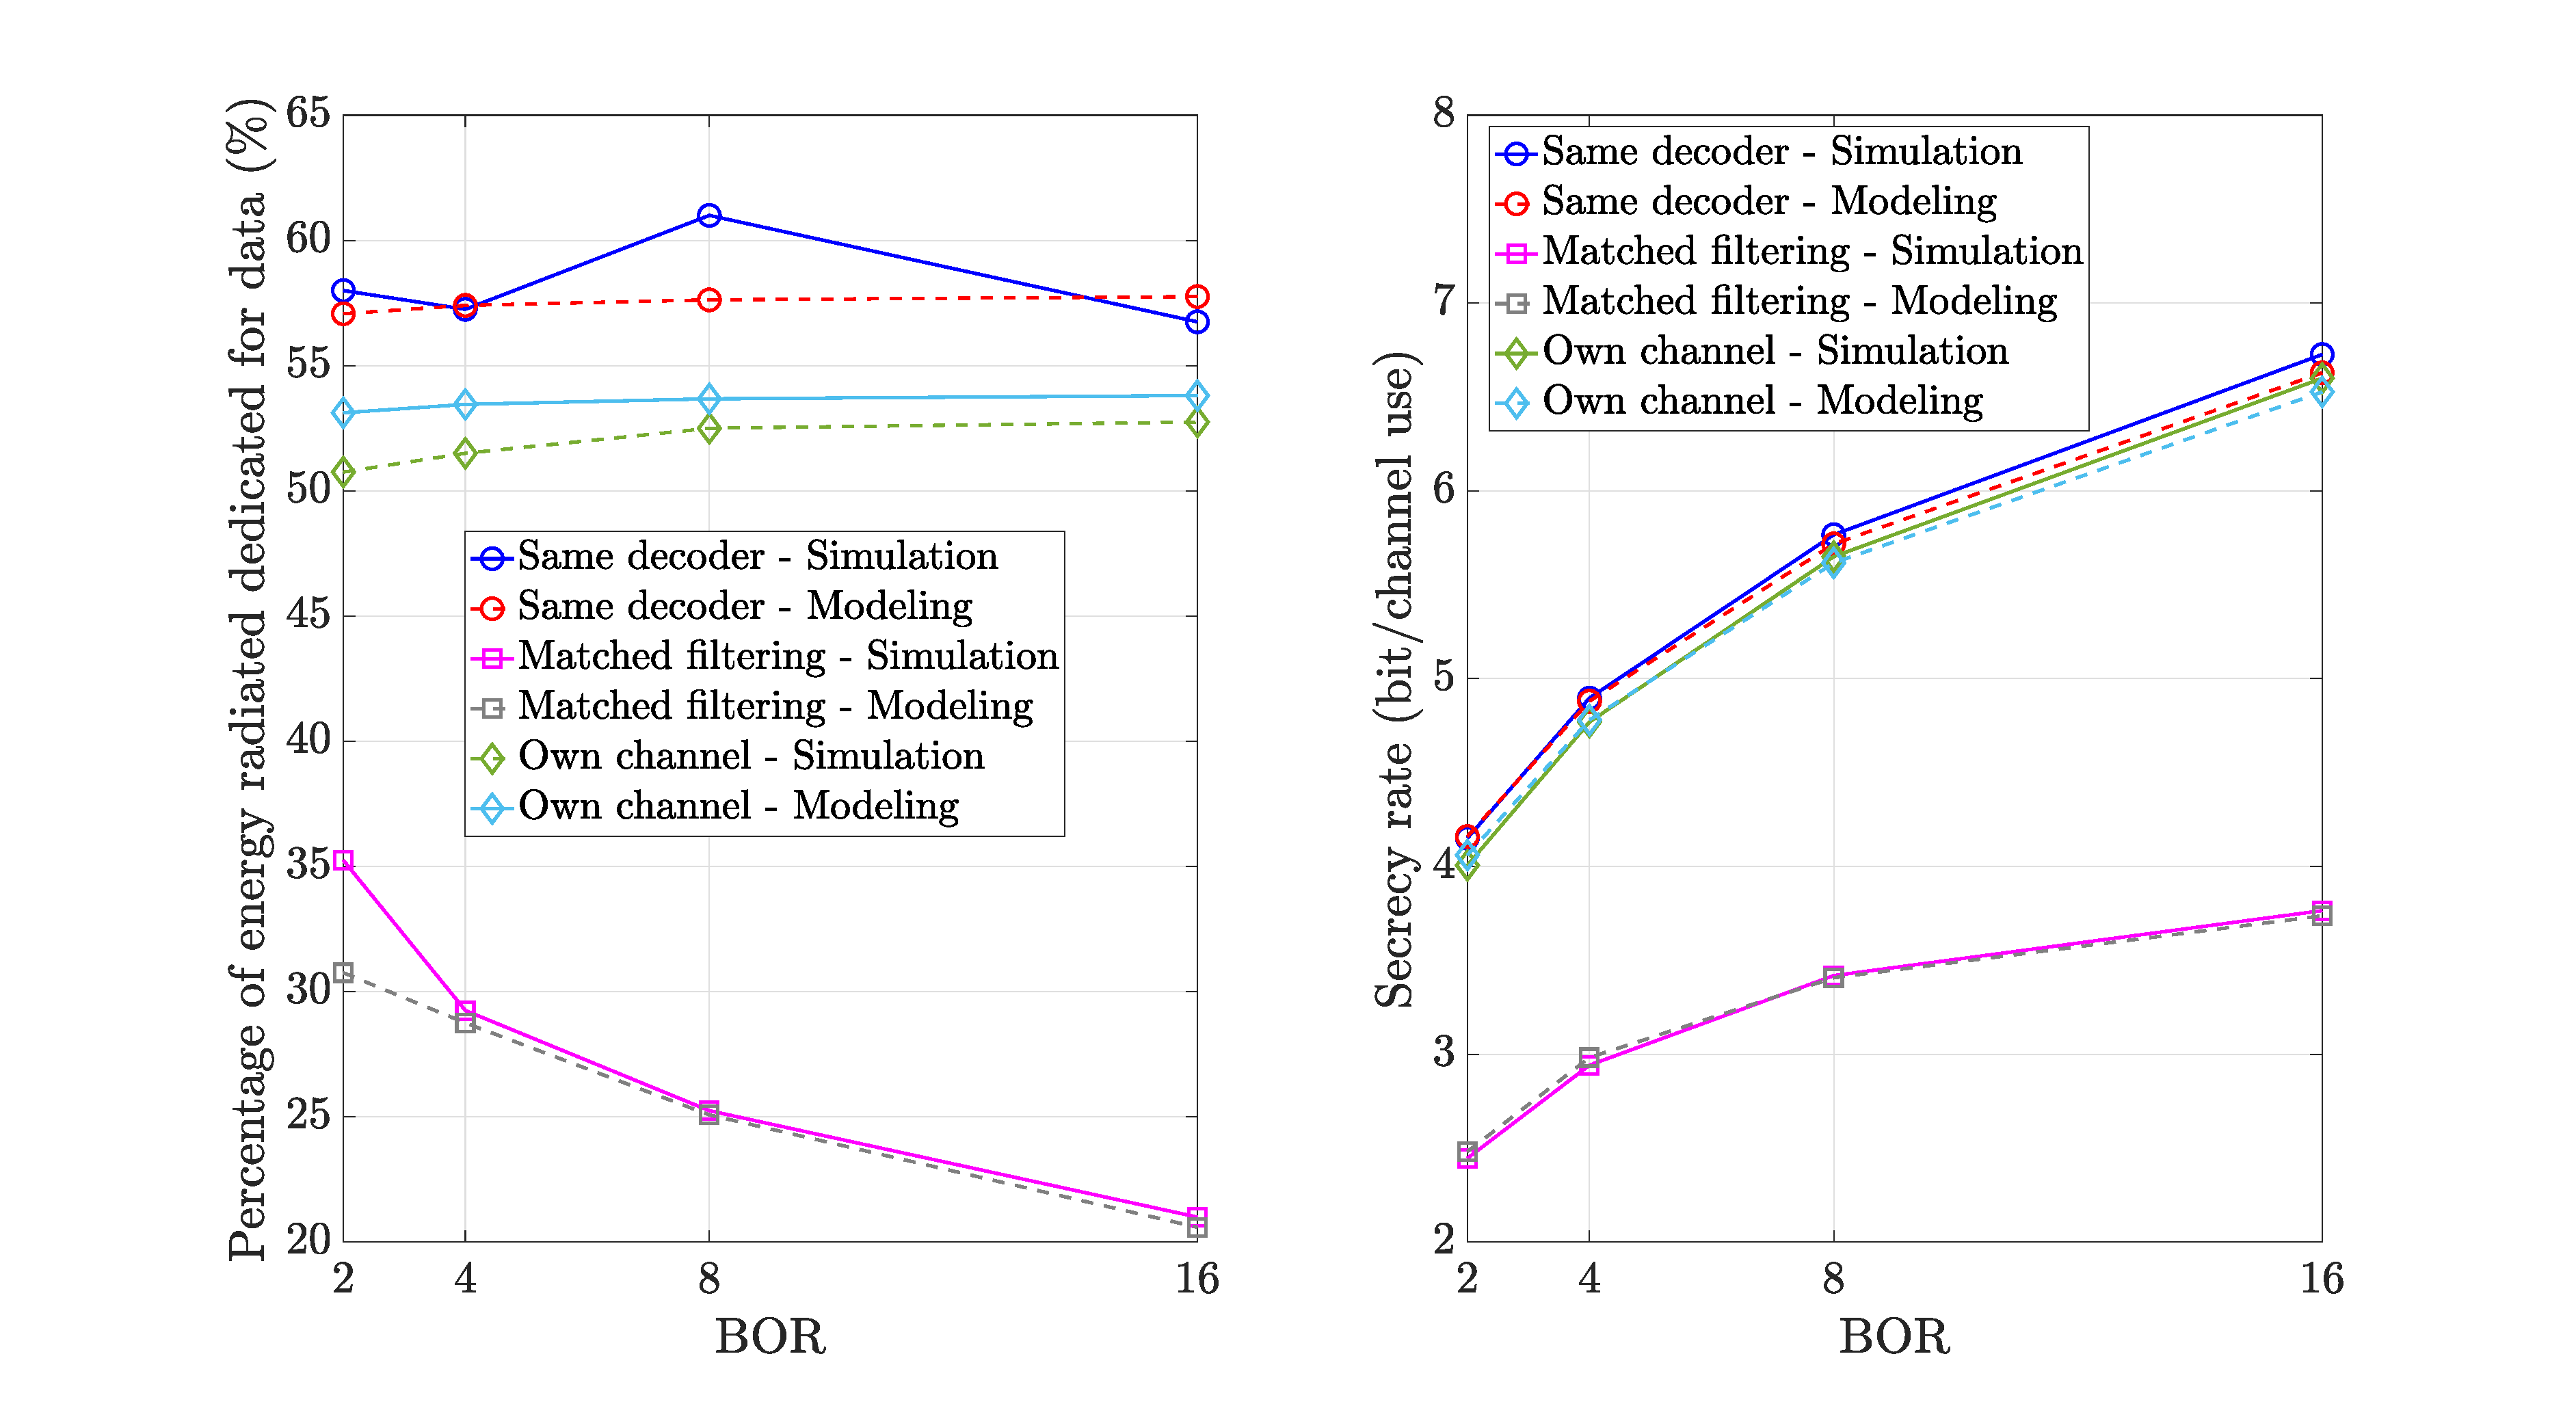
\includegraphics[width=1.1\linewidth]{graphs/SISO_no_corr_optimal_alpha_EbN0b_10_EbN0e_5.eps}
	\caption{Optimal of AN energy to inject, $E_b/N_0 = 10$dB at Bob,  $E_b/N_0 = 5$dB at Eve}
	\label{fig_optimalAN}
\end{figure}
The left part of Fig.\ref{fig_optimalAN} illustrates the values of $\alpha_{\text{opt}}$ given by (\ref{eq:optimal_alpha_decod_0}), (\ref{eq:optimal_alpha_decod_1}) and (\ref{eq:optimal_alpha_decod_5}) that maximize the  ergodic SR determined from the closed-form approximations (\ref{eq:SR_anal2_decod_0}), (\ref{eq:SR_anal2_decod_1}), and (\ref{eq:SR_anal2_decod_5}), as well as obtained from the numerical simulations, as a function of the BOR. The analytic estimations of the optimal amount of data energy to inject are not perfect but, the resulting simulated SR are very close to the maximal SR obtained numerically, as it can be observed on right part of Fig.\ref{fig_optimalAN}. The reason can be observed in Fig.\ref{fig_modelvssimu} where the SR curves vary very slowly about their maxima when $\alpha$ changes, for all models. So, for a given BOR value, Alice can make a rough determination of $\alpha_{\text{opt}}$ depending on Eve decoding structure, and therefore the available SR, if $E_b/N_0$ is known. One can also note that much lower values of $\alpha_{\text{opt}}$ should be injected to maximize the SR when Eve matched filters the received signal compared to the two other scenarios.


\begin{figure}[h!t]
	\centering
	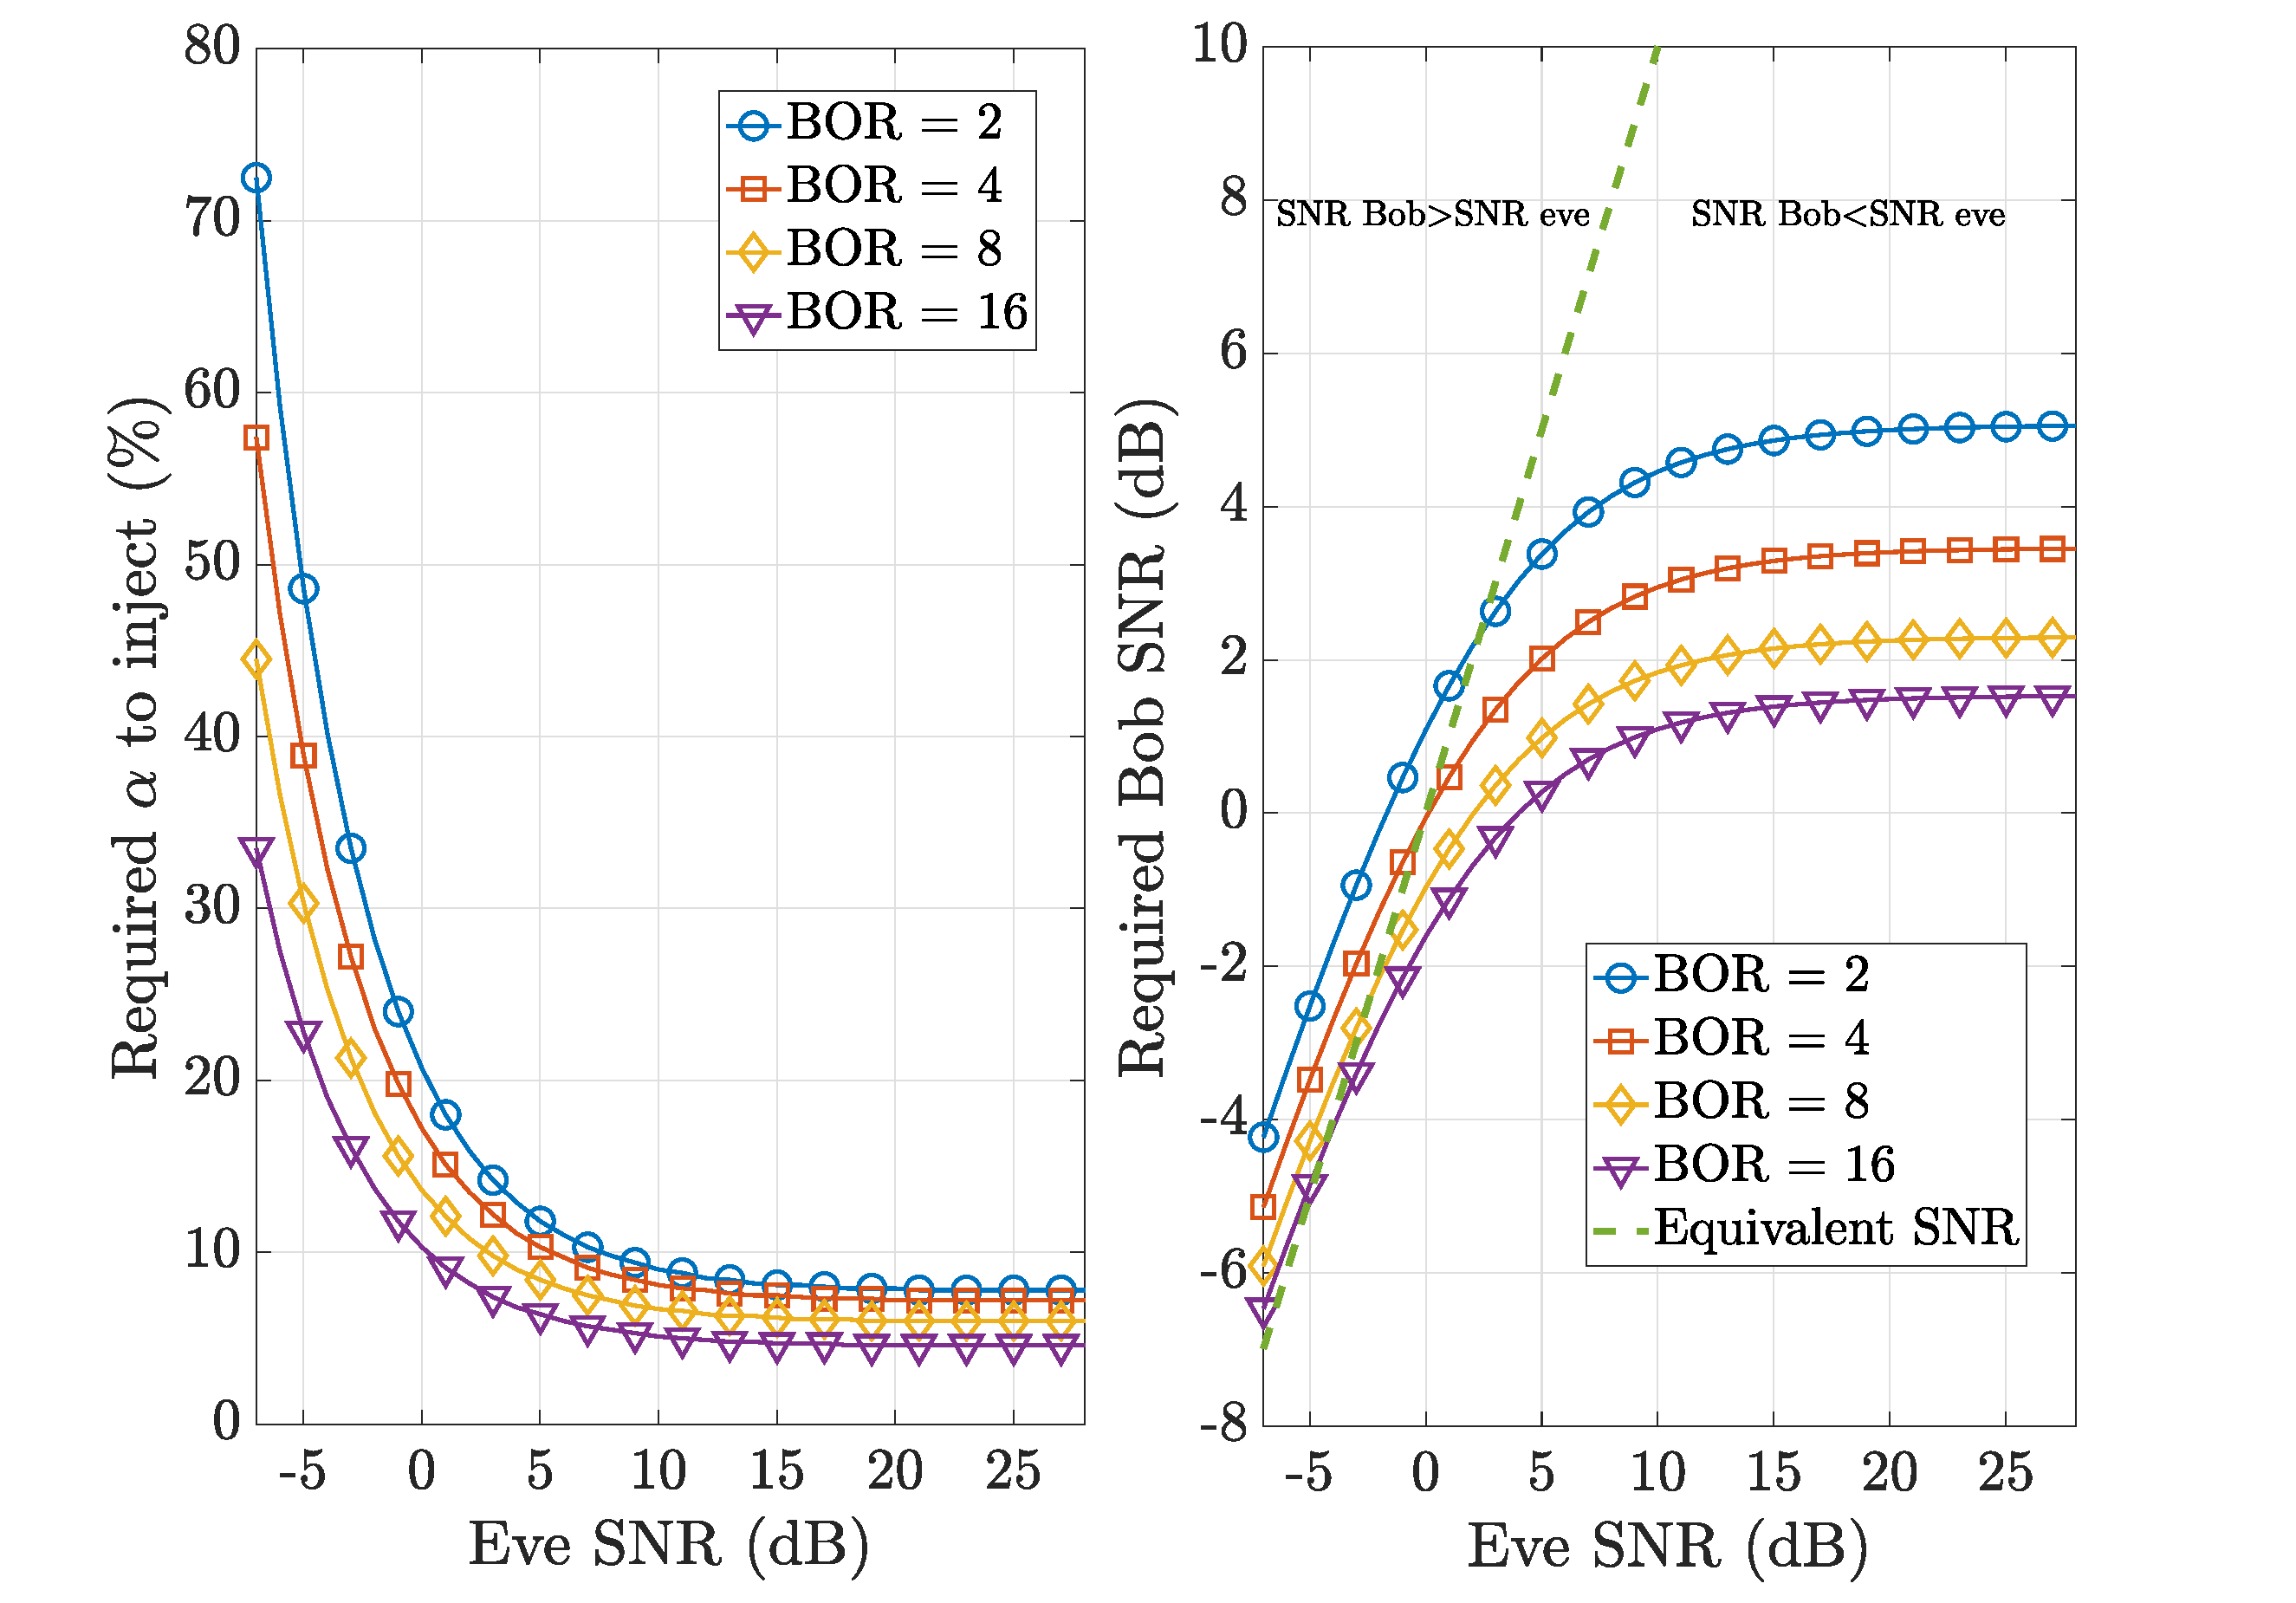
\includegraphics[width=1\linewidth]{graphs/SISO_no_corr_targettedSR_0_model2.eps}
	\caption{Targetted SR = 0 bit/channel use, matched filtering at Eve}
	\label{fig_targettedSR}
\end{figure} 
Fig.\ref{fig_targettedSR} illustrates the discussion from section \ref{sec:required-snr-at-bob-for-a-targetted-sr}, only for the scenario where Eve implements a matched filter. A SR larger than 0 bit per channel use is targetted in order to investigate under which conditions a positive secrecy can be ensured with the proposed FD TR SISO OFDM precoder scheme.

The left part of Fig.\ref{fig_targettedSR} shows the required amount of data energy to inject to target the SR, as a function of Eve's SNR for different BOR values. One can observe that more AN energy must be injected when Eve SNR increases, which highlights once again  the importance of the AN addition. In addition, we observe that higher values of $\alpha$ are needed for lower BOR values, which could have been anticipated from Fig.\ref{fig_optimalAN}

The right part of Fig.\ref{fig_targettedSR} represents the required SNR values at Bob. First, one observes that, except for low Eve SNRs, i.e., high AWGN energies, lower SNR values at Bob than at Eve are required in order to achieve a positive SR. We see that Bob SNR curves lay in the right side of the green dotted curve as soon as Eve's SNR is higher than 3dB, for all BOR values. The green dotted curve represents the set of points where Bob and Eve SNRs are identical, i.e., where Bob and Eve channels are equivalently degraded. In particular, for high SNR values at Eve, typically higher than 15dB, we note a saturation of Bob required SNR, for all BOR values. This highlights that positive secrecy can be obtained with our FD TR SISO OFDM precoder even if Bob's channel is a degraded version of the wiretap link. Finally, higher Bob SNR values are required when the BOR decreases. This is explained by the fact that the frequency diversity gain decreases with a decrease of the BOR value. Consequently, a better channel condition is needed to target the same SR 
%%


\subsection{Waterfilling optimization performances}
{\color{red}  ATTENTION: REFAIRE SIMU + LONGUE AU LABO}

\begin{figure}[h!t]
	\centering
	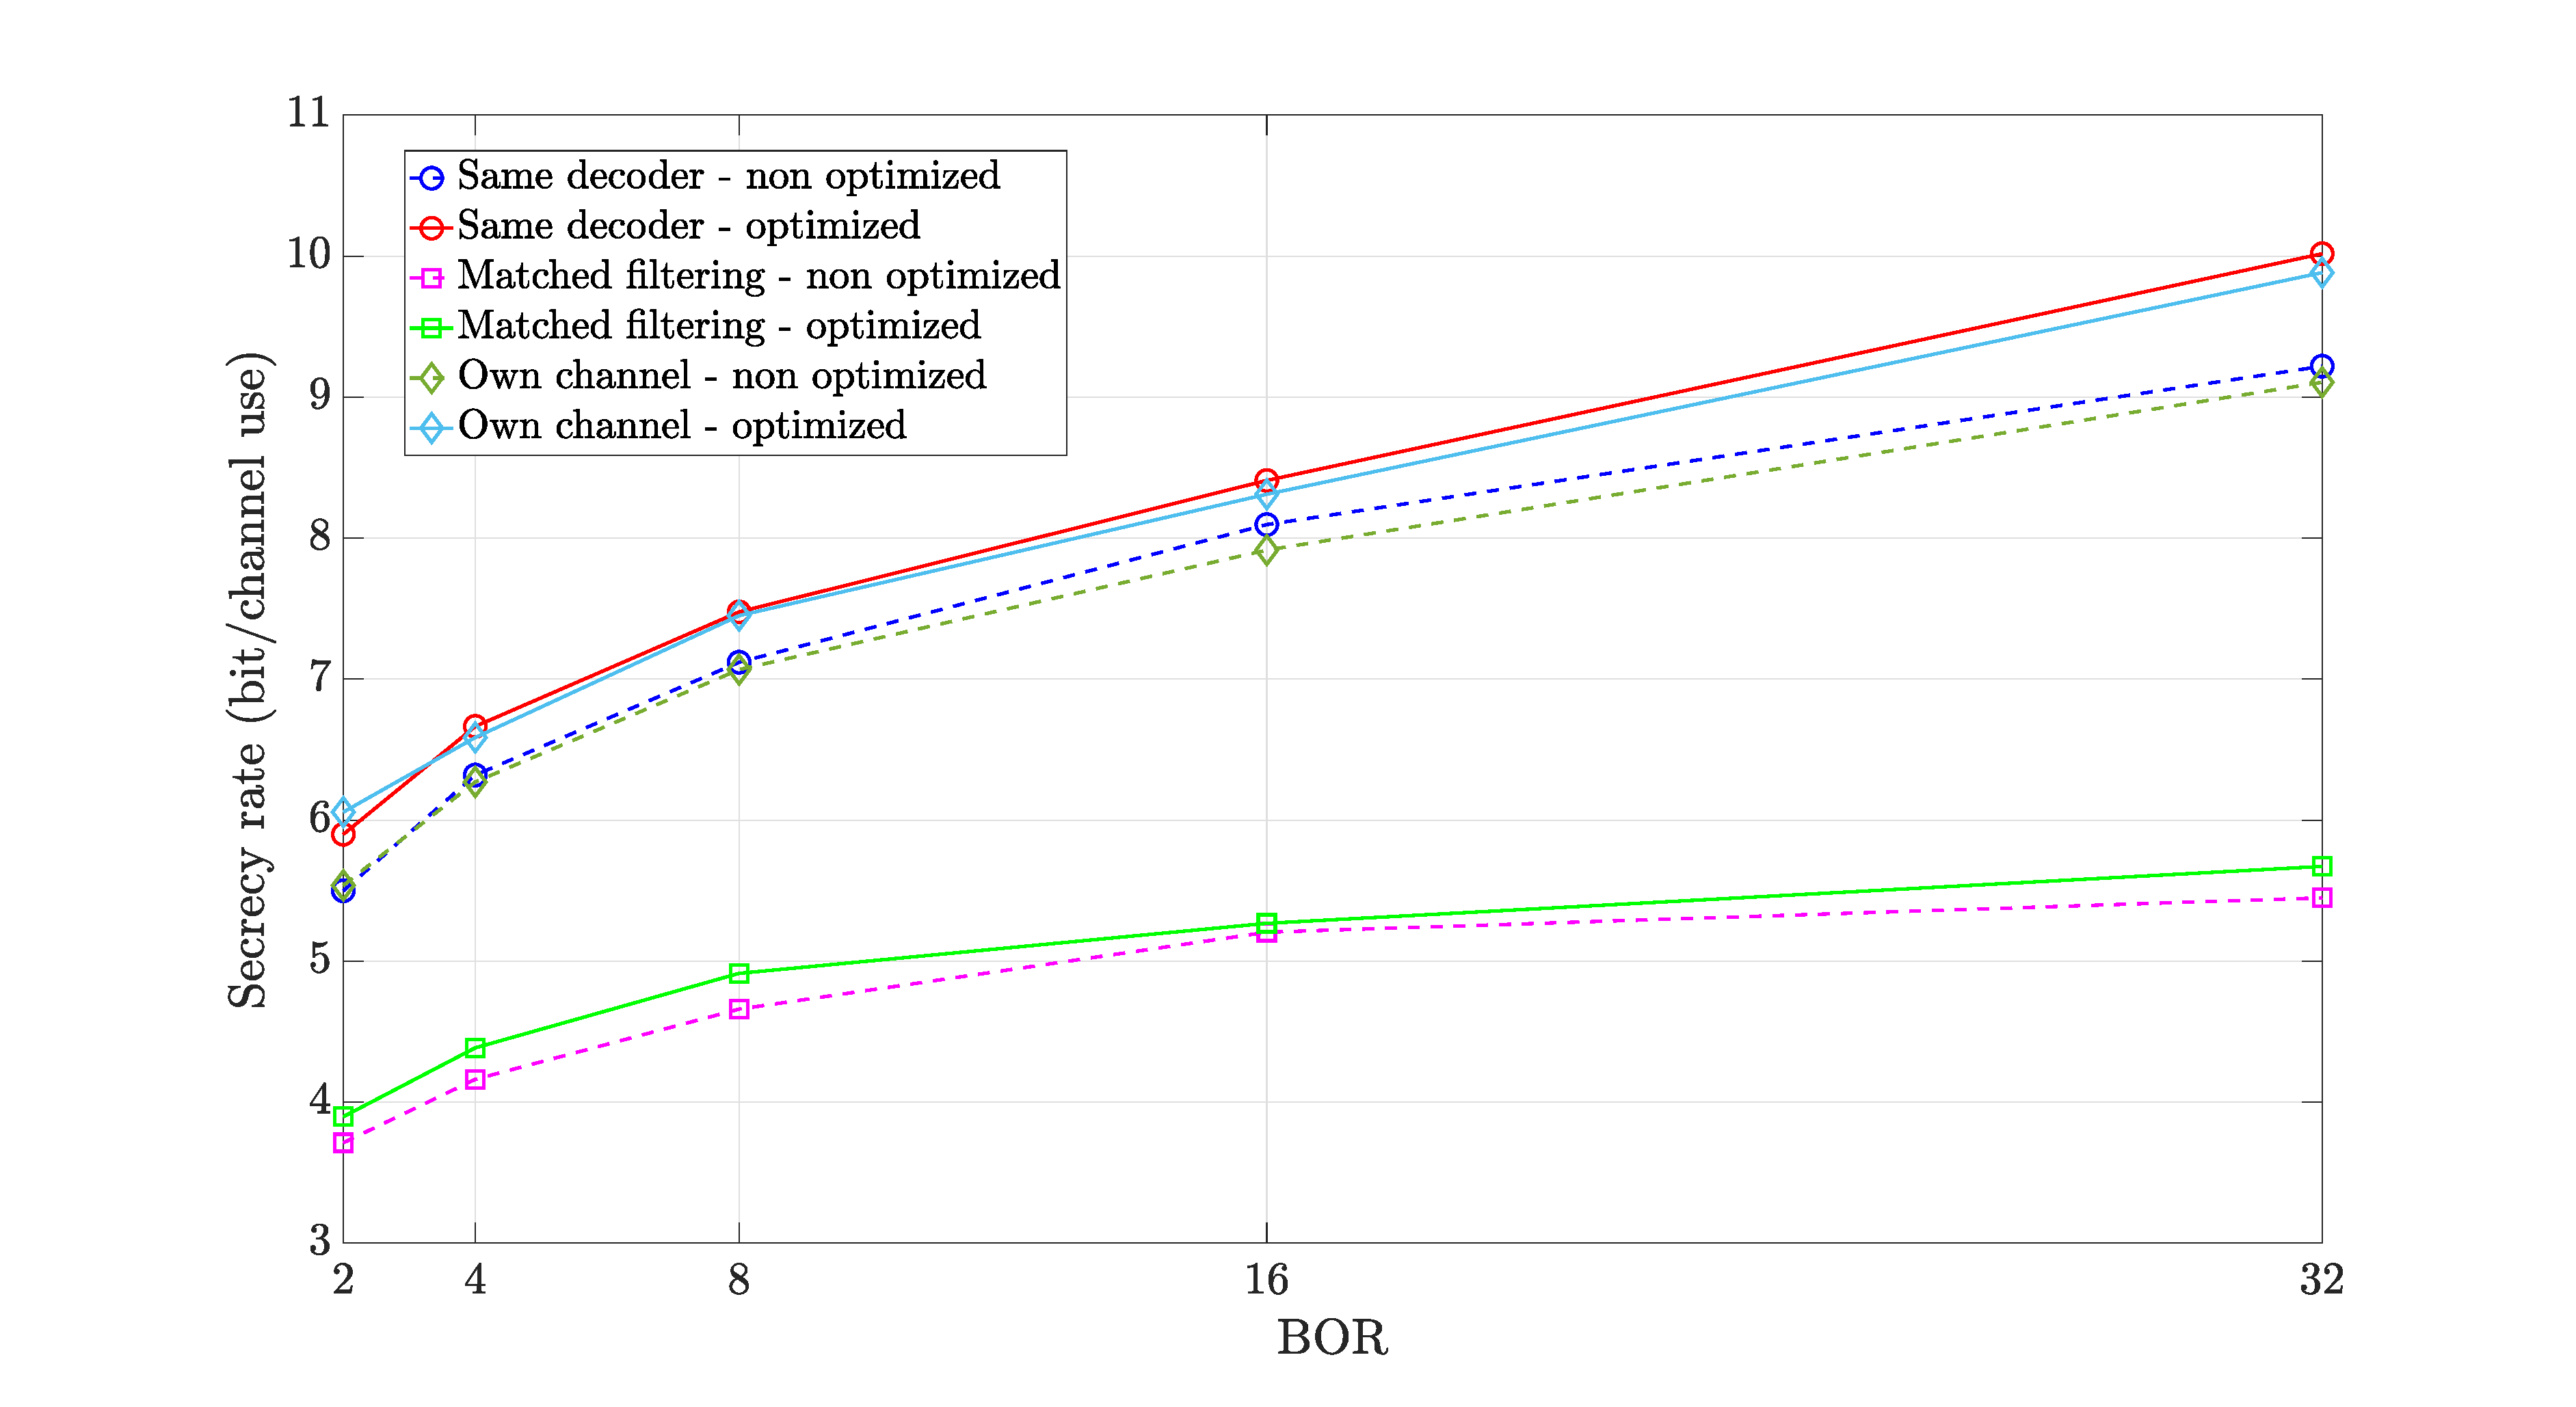
\includegraphics[width=1\linewidth]{graphs/SISO_no_corr_waterfilling.eps}
	\caption{Waterfilling optimization, $E_b/N_0 = 15$dB at Bob and Eve, BOR = 4}
	\label{fig_waterfilling_opt}
\end{figure}
Fig. \ref{fig_waterfilling_opt} presents the maximal values of the SR for the three decoding structures, before (dotted lines) and after (continuous lines) waterfilling optimization. As a reminder, before and after optimization, the mean energy radiated dedicated to the useful data remains unchanged, and the AN signal always remains in Bob's null space. The optimal amount of data energy to inject is computed thanks to (\ref{eq:optimal_alpha_decod_0}), (\ref{eq:optimal_alpha_decod_1}) and (\ref{eq:optimal_alpha_decod_5}) in order to ensure a maximal ergodic SR. The SR is then further increased via the waterfilling optimization procedure, as described in section \ref{subsec:perf_waterf}. As we can see, there is an increase of the SR for all three models and all BOR values thanks to the waterfilling. 

%%%%%%%%%   CONCLUSONS   %%%%%%%%% 
\section{Conclusions}\label{sec:conclusions}
In this paper, the problem of securing the FD TR SISO OFDM wireless transmission, in a FF environment, from a transmitter to a legitimate receiver in the presence of a passive eavesdropper is considered. A novel and original approach based on the addition of an AN signal onto OFDM blocks that improves the PLS is proposed. This approach can be easily integrated into existing standards based on OFDM. It only requires a single transmit antenna and is therefore well suited for devices with limited capabilities. Three different decoding structures for the passive eavesdropper are considered, resulting from the handshake procedure between Alice and Bob. Analytic and simulation results show that the novel approach significantly improves the security of the communication and so considerably jeopardizes any attempt of an eavesdropper to retrieve the data.






%\begin{table}[!t]
% increase table row spacing, adjust to taste
%\renewcommand{\arraystretch}{1.3}
%\caption{An Example of a Table}
%\label{table_example}
%\centering
% Some packages, such as MDW tools, offer better commands for making tables
% than the plain LaTeX2e tabular which is used here.
%\begin{tabular}{|c||c|}
%\hline
%One & Two\\
%\hline
%Three & Four\\
%\hline
%\end{tabular}
%\end{table}






%\newpage


%%%%%%%%%   APPENDICES  %%%%%%%%% 
\appendices
\section{SINR derivation}\label{sec:sinr-derivation-app}


\subsection{At the intended position}
\subsubsection{Data term}\label{sec:data-term-app}
\begin{equation}
	\begin{split}
		\EX{|B_1|^2} =& \EX{\module{\sqrt{\alpha} \; \spread^H \module{\HB}^2 \spread}^2} \\
		\EX{|B_{1,n}|^2} =&\EX{\left|\frac{\sqrt{\alpha}}{U}\sum_{i=0}^{U-1} \left| h_{\text{B}, n + iN}\right|^2\right|^2}  \\
		=& \frac{\alpha}{U^2} \EX{\left(\sum_{i=0}^{U-1} \left| h_{\text{B}, n + iN}\right|^2\right) \left(\sum_{j=0}^{U-1} \left| h_{\text{B}, n + jN}\right|^2\right)^H}\\
		=&  \frac{\alpha}{U^2} \Big(\EX{\sum_{i=0}^{U-1}\left| h_{\text{B}, n + iN}\right|^4} +\\
		& \EX{\sum_{i=0}^{U-1}\left| h_{\text{B}, n + iN}\right|^2}\EX{\sum_{\substack{j=0 \\ j\neq i}}^{U-1} | h^*_{\text{B}, n + jN}|^2} \Big) \\
		=& \frac{\alpha}{U^2} \left( 2U + U(U-1)\right) = \frac{\alpha (U+1)}{U}
	\end{split}
	\label{eq:appA:data_bob-app}
\end{equation}
where we used the fact that $\EX{\left| h_{\text{B}, n + iN}\right|^2} = 1$ and $\EX{\left| h_{\text{B}, n + iN}\right|^4} = 2$ since $\HB \sim \mathcal{CN}(0,1)$.



\subsubsection{AWGN term}\label{sec:awgn-term-app}
\begin{equation}
	\begin{split}
		\EX{|B_2|^2} &=  \EX{\module{\spread^H \vb}^2} \\
		&= \EX{\left(\spread^H \vb \right)\left(\spread^H \vb \right)^H} \\
		&=\EX{\spread^H \vb \vb^* \spread } \\
		\EX{|B_{2,n}|^2} &= \frac{1}{U} \EX{\sum_{i=0}^{U-1} |v_{\text{B}, n + iN}|^2} = \sigma^2_{\text{V,B}}
	\end{split}
	\label{eq:appA:noise_bob-app}
\end{equation}





\subsection{At the unintended position}\label{sec:at-the-unintended-position-app}
\subsubsection{Same decoding structure as Bob}\label{sec:same-decoding-structure-as-bob-app}
\paragraph{Data term}\label{sec:data-term-app-1}
\begin{equation}
	\begin{split}
		\EX{|\textbf{E}_{1}|^2} &= \EX{\module{\sqrt{\alpha}\spread^H \HE\HB^* \spread}^2} \\
		\EX{|E_{1,n}|^2}&=\alpha \EX{\frac{1}{U^2} \sum_{i=0}^{U-1} \left| h_{\text{E}, n + iN} \right|^2 \left| h^*_{\text{B}, n + iN}\right|^2 } \\
		&= \frac{\alpha}{U}
	\end{split}
	\label{eq:appA:data_eve_filt0-app}
\end{equation}



\paragraph{AWGN term}\label{sec:awgn-term-app-1}
\begin{equation}
	\begin{split}
		\EX{|\textbf{E}_{2}|^2} &=  \EX{\module{\spread^H \ve}^2} \\
		&=\EX{\spread^H \ve \ve^* \spread } \\
		\EX{|E_{2,n}|^2} &= \frac{1}{U} \EX{\sum_{i=0}^{U-1} |v_{\text{E}, n + iN}|^2} = \sigma^2_{\text{V,E}}
	\end{split}
	\label{eq:appA:noise_eve_filt0-app}
\end{equation}


\paragraph{AN term}\label{sec:an-term-app-1}
\begin{equation}
	\begin{split}
		\EX{|\textbf{E}_{3}|^2} &=  \EX{\module{\sqrt{1-\alpha}\spread^H \HE \w}^2} \\
		&=(1-\alpha)\EX{\spread^H \HE\textbf{H}^*_{\text{E}} \w\w^* \spread } \\
		\EX{|E_{3,n}|^2}  &= \frac{1-\alpha}{U} \EX{\sum_{i=0}^{U-1} |h_{\text{E}, n + iN}w_{n + iN}|^2} = \frac{1-\alpha}{U}
	\end{split}
	\label{eq:appA:an_eve_filt0-app}
\end{equation}

\subsubsection{Matched filtering}\label{sec:matched-filtering-app}
\paragraph{Data term}\label{sec:data-term-app-2}
\begin{multline}
	\EX{|E_{1,n}|^2} = \alpha \EX{\left|\frac{1}{U}\sum_{i=0}^{U-1} \left| h_{\text{B}, n + iN}\right|^2 \left| h_{\text{E}, n + iN}\right|^2\right|^2} \\
	=\frac{\alpha}{U^2} \mathbb{E} \Bigg[\sum_{i=0}^{U-1} \left| h_{\text{B}, n + iN}\right|^4 \left| h_{\text{E}, n + iN}\right|^4 \\
	+ \sum_{i=0}^{U-1}\sum_{\substack{j=0 \\ j\neq i}}^{U-1}  \left| h_{\text{B}, n + jN}\right|^2 \left| h_{\text{E}, n + iN}\right|^2 \left| h^*_{\text{B}, n + iN}\right|^2 \left| h^*_{\text{E}, n + jN}\right|^2 \Bigg] \\
	= \frac{\alpha}{U^2} \left(U.2.2 + U(U-1) \right) = \frac{\alpha (U+3)}{U}
	\label{eq:data_eve_filt1-app}
\end{multline}
where we used the fact that $\EX{\left| h_{\text{E}, n + iN}\right|^2} = 1$ and $\EX{\left| h_{\text{E}, n + iN}\right|^4} = 2$ since $\HE \sim \mathcal{CN}(0,1)$.



\paragraph{AWGN term}\label{sec:awgn-term-app-2}
\begin{equation}
	\begin{split}
		\EX{|\textbf{E}_{2}|^2} &=  \EX{\module{\spread^H \HE^* \HB \ve}^2} \\
		&=\EX{\spread^H   \HE \HE^* \HB\HB^*  \ve \ve^* \spread } \\
		\EX{|E_{2,n}|^2} &= \frac{1}{U} \EX{\sum_{i=0}^{U-1} |h_{\text{E}, n + iN}|^2 |h_{\text{B}, n + iN}|^2 |v_{\text{E}, n + iN}|^2} = \sigma^2_{\text{V,E}}
	\end{split}
	\label{eq:noise_eve_filt1-app}
\end{equation}

\paragraph{AN term}\label{sec:an-term-app-2}
The component $\textbf{A}_{3,n}$ depends on $\textbf{w}$ and $\HB$ which are correlated via the AN design (\ref{eq:an_cond}). The expectation is therefore more difficult to compute. After some mathematical operations, we find: {\color{red} JUSQU'A QUEL POINT METTRE LES DERIVATIONS ICI ? CA PREND 3 PAGES DANS LE RAPPORT}
\begin{equation}
	\EX{|E_{3,n}|^2} = \frac{1-\alpha}{U+1}
	\label{eq:an_eve_filt1-app}
\end{equation}


\subsubsection{Own channel knowledge}\label{sec:own-channel-knowledge-app}
\paragraph{Data term}\label{sec:data-term-app-3}
\begin{multline}
	\EX{|E_{1,n}|^2} = \alpha \EX{\left|\frac{1}{U}\sum_{i=0}^{U-1} h_{\text{B}, n + iN}^* \left| h_{\text{E}, n + iN}\right|^2\right|^2} \\
	=\frac{\alpha}{U^2} \mathbb{E}\Bigg[ \sum_{i=0}^{U-1} \left| h_{\text{B}, n + jN}\right|^2 \left| h_{\text{E}, n + iN}\right|^4 \\
	+ \sum_{i=0}^{U-1}\sum_{\substack{j=0 \\ j\neq i}}^{U-1}  h_{\text{B}, n + jN} h^*_{\text{B}, n + iN} \left| h_{\text{E}, n + jN}\right|^2 \left| h^*_{\text{E}, n + iN}\right|^2 \Bigg] \\
	= \frac{\alpha}{U^2} \left(U.2.1 + U(U-1).1.1.0\right) = \frac{2\alpha}{U}
	\label{eq:data_eve_filt5-app}
\end{multline}


\paragraph{AWGN term}\label{sec:awgn-term-app-3}
\begin{equation}
	\begin{split}
		\EX{|\textbf{E}_{2}|^2} &=  \EX{\module{\spread^H \HE^* \ve}^2} \\
		&=\EX{\spread^H   \left|\HE\right|^2  \left|\ve\right|^2 \spread } \\
		\EX{|E_{2,n}|^2} &= \frac{1}{U} \EX{\sum_{i=0}^{U-1} |h_{\text{E}, n + iN}|^2 |v_{\text{E}, n + iN}|^2} = \sigma^2_{\text{V,E}}
	\end{split}
	\label{eq:noise_eve_filt5-app}
\end{equation}

\paragraph{AN term}\label{sec:an-term-app-3}
\begin{equation}
	\begin{split}
		\EX{|\textbf{E}_{3}|^2} &=  \EX{\module{\sqrt{1-\alpha}\spread^H \left|\HE\right|^2 \w}^2} \\
		&=(1-\alpha)\EX{\spread^H \left|\HE\right|^2 \w\w^* \left|\HE^*\right|^2\spread } \\
		\EX{|E_{3,n}|^2}  &= \frac{1-\alpha}{U} \EX{\sum_{i=0}^{U-1} |h_{\text{E}, n + iN}|^4 |w_{n + iN}|^2} = \frac{2(1-\alpha)}{U}
	\end{split}
	\label{eq:an_eve_filt5-app}
\end{equation}

%\ifCLASSOPTIONcaptionsoff
%  \newpage
%\fi

%%%%%%%%%   BIBLIOGRAPHY   %%%%%%%%% 

%\newpage
\bibliographystyle{IEEEtran}
\bibliography{biblio} 


%%%%%%%%%   BIOGRAPHY   %%%%%%%%% 
%\begin{IEEEbiography}{Michael Shell}
%Biography text here.
%\end{IEEEbiography}

% if you will not have a photo at all:
%\begin{IEEEbiographynophoto}{John Doe}
%Biography text here.
%\end{IEEEbiographynophoto}


%\begin{IEEEbiographynophoto}{Jane Doe}
%Biography text here.
%\end{IEEEbiographynophoto}


\end{document}


